\documentclass[10pt]{article}\usepackage[]{graphicx}\usepackage[]{color}
% maxwidth is the original width if it is less than linewidth
% otherwise use linewidth (to make sure the graphics do not exceed the margin)
\makeatletter
\def\maxwidth{ %
  \ifdim\Gin@nat@width>\linewidth
    \linewidth
  \else
    \Gin@nat@width
  \fi
}
\makeatother

\definecolor{fgcolor}{rgb}{0.345, 0.345, 0.345}
\newcommand{\hlnum}[1]{\textcolor[rgb]{0.686,0.059,0.569}{#1}}%
\newcommand{\hlstr}[1]{\textcolor[rgb]{0.192,0.494,0.8}{#1}}%
\newcommand{\hlcom}[1]{\textcolor[rgb]{0.678,0.584,0.686}{\textit{#1}}}%
\newcommand{\hlopt}[1]{\textcolor[rgb]{0,0,0}{#1}}%
\newcommand{\hlstd}[1]{\textcolor[rgb]{0.345,0.345,0.345}{#1}}%
\newcommand{\hlkwa}[1]{\textcolor[rgb]{0.161,0.373,0.58}{\textbf{#1}}}%
\newcommand{\hlkwb}[1]{\textcolor[rgb]{0.69,0.353,0.396}{#1}}%
\newcommand{\hlkwc}[1]{\textcolor[rgb]{0.333,0.667,0.333}{#1}}%
\newcommand{\hlkwd}[1]{\textcolor[rgb]{0.737,0.353,0.396}{\textbf{#1}}}%
\let\hlipl\hlkwb

\usepackage{framed}
\makeatletter
\newenvironment{kframe}{%
 \def\at@end@of@kframe{}%
 \ifinner\ifhmode%
  \def\at@end@of@kframe{\end{minipage}}%
  \begin{minipage}{\columnwidth}%
 \fi\fi%
 \def\FrameCommand##1{\hskip\@totalleftmargin \hskip-\fboxsep
 \colorbox{shadecolor}{##1}\hskip-\fboxsep
     % There is no \\@totalrightmargin, so:
     \hskip-\linewidth \hskip-\@totalleftmargin \hskip\columnwidth}%
 \MakeFramed {\advance\hsize-\width
   \@totalleftmargin\z@ \linewidth\hsize
   \@setminipage}}%
 {\par\unskip\endMakeFramed%
 \at@end@of@kframe}
\makeatother

\definecolor{shadecolor}{rgb}{.97, .97, .97}
\definecolor{messagecolor}{rgb}{0, 0, 0}
\definecolor{warningcolor}{rgb}{1, 0, 1}
\definecolor{errorcolor}{rgb}{1, 0, 0}
\newenvironment{knitrout}{}{} % an empty environment to be redefined in TeX

\usepackage{alltt}
\usepackage{graphicx, verbatim}
\usepackage[utf8]{inputenc}
\usepackage{amsmath}
\usepackage{amssymb}
\usepackage{amscd}
\usepackage{lipsum}
\usepackage{blindtext}
\usepackage{todonotes}
\usepackage[tableposition=top]{caption}
\usepackage{ifthen}
\usepackage{caption}
\setlength{\textwidth}{6.5in} 
\setlength{\textheight}{9in}
\setlength{\oddsidemargin}{0in} 
\setlength{\evensidemargin}{0in}
\setlength{\topmargin}{-1.5cm}
\setlength{\parindent}{0cm}
\usepackage{setspace}
\usepackage{float}
\usepackage{fancyhdr}
\usepackage{tabularx}
\usepackage{soul} 

\usepackage{hyperref}
\hypersetup{
  colorlinks   = true, %Colours links instead of ugly boxes
  urlcolor     = blue, %Colour for external hyperlinks
  linkcolor    = blue, %Colour of internal links
  citecolor   = red %Colour of citations
}

\usepackage[backend=biber ,sorting=none]{biblatex}
\bibliography{references}
\begin{filecontents*}{references.bib}
\end{filecontents*}


%\fancyhf{}
\rfoot{Group 2 \thepage}
\singlespacing
\usepackage[affil-it]{authblk} 
\usepackage{etoolbox}
\usepackage{lmodern}

% \makeatletter
% \renewcommand{\maketitle}{\bgroup\setlength{\parindent}{16pt}
% \begin{flushleft}
%   \textbf{\@title}
% 
%   \@author
% \end{flushleft}\egroup
% }

%\renewcommand\Authfont{\fontsize{14}{18.4}\selectfont}
%\makeatother

% \pagestyle{fancy}
% \rfoot{Page \thepage}
 %\thispagestyle{empty} 



\IfFileExists{upquote.sty}{\usepackage{upquote}}{}
\begin{document}

\title{\LARGE Professional Development and Research Skills \\ CMM507 Coursework  \\ Group 2: Plastic Pollution in Oceans}

\author{ALEXANDER RITCHIE, \textit{\href{1911218@rgu.ac.uk}{1911218@rgu.ac.uk}};\\ GEORGIOS ORFANAKIS, \textit{\href{1903446@rgu.ac.uk}{1903446@rgu.ac.uk}};\\ KAREN JEWELL, \textit{\href{1415410@rgu.ac.uk}{1415410@rgu.ac.uk}};\\ ROSHI SHRESTHA, \textit{\href{1903445@rgu.ac.uk}{1903445@rgu.ac.uk}};\\ STUART WATT, \textit{\href{1501869@rgu.ac.uk}{1501869@rgu.ac.uk}}}

\maketitle
\noindent\rule{16cm}{0.4pt}


\section{Introduction}

\subsection{Problem Statement}\label{statement}

Plastic pollution is a serious problem in the marine environment which has major impact on marine and human health. To understand the depth of the problem, it is essential to understand the amount and composition of marine litter. This can help in applying various mitigation strategies. This section will include: \hl{should this talk about the section or the report? Do we need the problem statement???}
\begin{itemize}
\item An overview of marine pollution
\item Motivation behind this topic
\item Aim and objectives of this report
\end{itemize}


\subsection{Overview}\label{over}

Marine pollution is a major global issue which impacts on environment, economy and human health. Although marine pollution is caused by many different materials, plastics consist of 60-80\% of the marine litter. \hl{reference?} Plastic is made from synthetic organic polymer derived from polymerisation of monomers extracted from oil \hl{I think plastics is just a oil product, not gas - confirm}.\cite{DERRAIK2002} \cite{RIOS2007} Its lightweight feature and durability make it very suitable to make a range of products we use in our everyday life.\cite{BARNES2009} \cite{SIVAN2011} These same features are what makes plastic a major component of pollution, due to overuse and non-managed waste disposal systems internationally, contributing to 10\% of the waste generated worldwide.\cite{BARNES2009} Due to its buoyancy, plastic debris can be dispersed over long distances and they can persist for a long time \hl{and never decompose?}. Jambeck et al.,\cite{JAMBECK2015} reported that in 2010 alone, between 4.8 million to 12.7 million metric tons of plastics entered the ocean. Plastics are everywhere in the marine environment and urgent action is required to mitigate this problem and reduce its harmful impact.\cite{RIOS2007} \cite{ROCHMAN2015}


\subsection{Motivation}\label{mot}

The impact of plastic pollution on marine life has been reviewed extensively. \cite{GALL2015} \cite{KUHN2015} \cite{RYAN2015} \cite{WILLIAMS2019} Over 700 marine wildlife species are affected due to entanglement in plastic ropes or materials, and from ingestion of plastics in the ocean.\cite{GALL2015} Over 340 species of marine animals were found to be entangled. \cite{KUHN2015} \hl{what's the difference between the 700 and the 340?} Over time, plastic disintegrates into microplastics and nanoplastics which are easily consumed by fish and enter the human food chain. Plastics have been found in a third of fish caught in the UK which included popular fish such as cod, haddock, and mackerel. \cite{LUSHER2013} The impact and effects of plastic entering the human food chain are still being studied, but plastic toxicity and the occurrence of microplastics and nanoplastics in the water supply also directly impacts human health, in addition to the contamination of seafood.\cite{ROCHMAN2015} \cite{MARKIC2020} \\

Although plastic litter has been a major cause of marine pollution for a while, its seriousness has only been realised recently and reducing plastic pollution has become a global aim. Research on plastic pollution in marine environments has played a big role in efforts to reduce it as well as in raising awareness globally. In order to understand plastic pollution in marine environments and its effects in the long term, it is essential to keep collecting data on patterns of marine debris around the world. Effective monitoring of plastic debris is essential to reducing the abundance of plastic debris everywhere. In addition, monitoring the type, frequency and the source of the litter is also important for marine pollution prevention initiatives. Most monitoring is done by survey, where organisations and volunteers record the types and frequencies of litter observed on the shoreline.\cite{COE1997} Litter is most abundant close to urban areas where beach visitor numbers are high.\cite{GARRITY1993}


\subsection{Objectives }\label{obj}

The main objectives of this project is outlined as follows:
\begin{itemize}	
\item To review available literature on marine plastic problems and their impacts
\item	To look at a suitable dataset to understand the composition of plastic pollution 
\item	To present the derived results and conclusions 
\end{itemize}

























\pagebreak
\section{Research}\label{research}

An integral part of this report required that the authors conducted a literature search to identify how researchers have been trying to monitor coastal pollution and find the problems associated with it. Several studies have reported the abundance of plastic as a coastal litter through scientific survey and citizen science methods. A 12-year observation of coastal debris pollution using citizen science in Taiwan revealed that most debris items found were plastic. \cite{WALTHER2018} 19 categories of debris items were collected during the clean-up events and the five most commonly recorded debris categories were: plastic shopping bags, plastic bottle caps, disposable tablewares, fishing equipment, and plastic drinking straws. There have been many other studies around the world regarding littering of the shores. In a study covering western Japan and the eastern coasts of Russia \cite{KUSUI2003}, it found that 55\% to 93.4\% of items over the Japanese shores were plastic, and the second most abundant item was resin pellet which is also a form of plastic. On the eastern Russian coast, plastic items were also the most abundant, contributing to approximately 55\% of all litter, mostly of plastic fragments. The composition of litter was similar in the two countries, although the concentration \hl{proportion?} of plastics was much higher in Japan. \cite{KUSUI2003} Further along the Asian upper east coast, hard plastic and styrofoam were the dominant plastic types found on Korean beaches. On average, hard plastic and styrofoam comprised 32\% and 48.5\% of the total debris count respectively. \\

In an older study over the Caribbean region, the most common types of debris found on the Caribbean coast of Panama were plastic and styrofoam, with the plastics being household or consumer related. Styrofoam packing materials were also abundant and may have come from trans-shipment activities of Colon's Free Zone, household waste, or offshore activity \cite{GARRITY1993}. A 2016/2017 annual study of 8 beaches in Tenerife in the Canary Islands also found that plastic was the most abundant litter there. They also reported that there was more accumulated plastic debris in remote beaches compared to the beaches near the city \hl{ which contradicts (or if supported by) the GARRITY1993 study "Litter is most abundant close to urban areas where beach visitor numbers are high"}, indicating that more debris were transported by tides. More long term study is required to understand the changes in the results reported over time. \cite{REINOLD2020} \\

It was observed by the authors of this report, that there are variations in how studies of litter accumulation have been conducted. The variations are present in the time span of the research, the parts of the coast from which litter was collected, as well as in the categorisation of litter, which creates difficulty when researchers want to compare different studies. The plastic pollution problem essentially requires the ability to assess changes in accumulation rates and composition, trends over time and the effectiveness of management systems, which is a hard task without good monitoring methodologies. Although monitoring of marine litter is currently carried out within a number of countries around the world, the methods of survey and monitoring used tend to be very different, preventing comparisons and harmonisation of data across regions or time. \\

This is why the scientific community has been trying to create some common ground, which has led to initiatives joined by many countries worldwide. One of these initiatives, and probably the most important, is the International Clean Coast (ICC) program which is a new, long term approach to cleaner beaches by using various activities to increase public awareness. \cite{ CHESHIRE2009} This initiative aims to develop a comprehensive litter characterisation scheme that uses both material composition and form. This allows Litter Monitoring Repeated \hl{os LMR a name? should it be encased in ""?} surveys of beaches, sea bed and/or surface waters to determine litter quantities such that information can be compared with baseline data to identify if changes occur over time or in response to management arrangements. \\

The ICC uses specifically developed categorisations of coast litter, with the most accepted being the Clean Coastal Index (CCI) protocol, which is useful for its simplicity and information provided, allowing comparisons between different times and places. The CCI protocol is different from most others \hl{other....protocols, systems?} having a focus on operational clean-up of beaches as well. The CCI is the recommended tool for evaluation of actual coast cleanliness, measuring plastic debris as an indicator of beach cleanliness, in an easy way \hl{easy for volunteers?} which precludes bias by the assessor. The CCI also proved to be a useful tool for measuring progress and the success of activities in raising awareness among the general public. \cite{ALKALAY2007} \\

A study in Israel followed the CCI protocol and found that plastic was the most ubiquitous \hl{prevalent, common?} beach litter item. An important contribution to this study was the ability to compare its findings to other Mediterranean beaches, showing that plastic might be \hl{is/was?} the dominant pollutant in the region, and non-plastic litter being highly specific to the region and cannot be treated universally. \cite{PORTMAN2017} In another study on litter pollution in a region of India, once again following the CCI protocol for the categorisation of litter, found that plastic was the main form of litter at approximately 45\% of total litter. Plastic bags topped the index at 33\%, followed by food wrappers, then plastic cups, and cigarette/cigar tips amounting to 5.5\%. \cite{KUMAR2016} The use of the common protocol in these two studies allows for researchers to compare their findings and create common plastic pollution models, even though the two coasts are continents apart. \\

Another study conducted in Cadiz, on the other side of the Mediterranean from Israel, found that plastic bottles and containers were the most frequent littered items, followed by plastic bags. This research also pointed out that surveys are heavily affected by clean-ups performed at beaches. \cite{WILLIAMS2016} Even though this study reaches important conclusions on ways to clean coasts the correct way, it cannot be easily compared, or its conclusions easily applied even with the case of the study in Israel sharing the Mediterranean Sea. \hl{because it is not using the CCI?}  \\

From this review, it is evident that there have been many studies conducted to monitor marine pollution in varying ways. One of the cost effective and easy method \hl{is it not the most cost-effective and easiest?} is the use of citizen science in which the public records any observations of marine litter. As discussed before, observations not following a standard protocol with proper guidance could be uncomparable and rendered ineffective. The Marine Debris Tracker (MDT) initiative \hl{can we mention who created/sponsored it?} was started in 2010 in North America and continues to operate today. The MDT allows anyone to record the marine debris observed, using an application on a mobile phone. The only report using data from this application is a web-based report by Tablada in 2018 \cite{JAMBECK2015B}, where data analysis was performed on 8 years of the data, mainly focused on North America. The study also concluded that plastic was the main type of debris recorded, with cigarettes being the top identified littered item. The subsequent sections of this report will aim to contribute to this body of knowledge, using the worldwide coastal littering dataset from the MDT, with an interest in identifying if plastic is indeed the most abundant litter of the worldwide dataset, which would be in agreement with the various studies discussed in this review. Following which, this report will analyse the distribution of subclasses within the plastics found, and explore if there could be a way to computationally monitor and assess the coastal littering problem, using the established CCI categorisation of litter. \\
















\pagebreak
\section {Methods}\label{methods}

\subsection{Dataset Description}\label{dataset}

The data used in this report was gathered using secondary data collection methods only. The authors did not collect or create any new data using primary methods. The data was downloaded from the Marine Debris Tracker website (www.marinedebris.engr.uga.edu) on \hl{what was the date of download?}. The dataset is composed of global observations from the start of the program in 2010 to the latest available date in February 2020. \\

As discussed in the section before, the MDT is a citizen science project where organisations or individuals can record observations of marine debris using a mobile phone application. \cite{JAMBECK2015B} The user records the observation using a structured form, and chooses the category of debris from a list provided, but there are also multiple available fields to populate including non-mandatory fields, and some allowing free text entry. An example of a non-mandatory field are "Lists"  which are user customisable groupings for listing their own collection of records.The table below describes the structure of the data. 

\begin{table}[H]
\begin{tabular}{ l l l }
Field & Description & Mandatory \\
\hline
ListName & customised groupings of records & Non-mandatory \\
ListID & ID for ListName & Non-mandatory \\
ItemName & the category of debris & Mandatory \\
ItemID & ID for ItemName & Non-mandatory \\
LogID & Unique ID for the observation & Non-mandatory \\
Quantity & number of pieces of debris observed & Mandatory \\
Error radius & radius around the site within the error for reasonable doubt & Mandatory \\
Latitude & coordinates of the location where the observation was made & Mandatory \\
Longitude & coordinates of the location where the observation was made & Mandatory \\
Altitude & coordinates of the location where the observation was made & Mandatory \\
Location & free-text description of the area the observation was made in & Non-mandatory \\
Description & free-text description for the observation & Non-mandatory \\
MaterialDescription & the material the debris was composed of & Mandatory \\
MaterialID & ID for MaterialDescription & Mandatory \\
Time & the date and time of observation & Non-mandatory \\
\end{tabular}
\end{table}


\pagebreak
\subsection{Dataset Pre-processing}

\begin{knitrout}\small
\definecolor{shadecolor}{rgb}{0.969, 0.969, 0.969}\color{fgcolor}\begin{kframe}
\begin{alltt}
\hlkwd{library}\hlstd{(tidyverse)}
\hlkwd{library}\hlstd{(purrr)}
\hlkwd{library}\hlstd{(magrittr)}
\hlkwd{library}\hlstd{(treemap)}
\hlkwd{library}\hlstd{(mapdata)}
\hlkwd{library}\hlstd{(viridis)}
\hlkwd{library}\hlstd{(lubridate)}
\hlkwd{library}\hlstd{(imager)}
\hlkwd{library}\hlstd{(xtable)}
\hlkwd{library}\hlstd{(dplyr)}


\hlstd{data} \hlkwb{<-} \hlkwd{list.files}\hlstd{(}\hlkwc{path} \hlstd{=} \hlstr{"data/debris/"}\hlstd{,} \hlkwc{full.names} \hlstd{=} \hlnum{TRUE}\hlstd{)} \hlopt
  \hlkwd{lapply}\hlstd{(}\hlkwc{FUN} \hlstd{= read_csv,} \hlkwc{col_types} \hlstd{=} \hlstr{"ififidddddcfcif"}\hlstd{)} \hlopt
  \hlkwd{reduce}\hlstd{(rbind)}
\end{alltt}
\end{kframe}
\end{knitrout}



From download, the data was cleaned to prepare it for analysis. \\

First, the datetime information was converted into a date type format and renamed as variable \textbf{Time}

\begin{knitrout}\small
\definecolor{shadecolor}{rgb}{0.969, 0.969, 0.969}\color{fgcolor}\begin{kframe}
\begin{alltt}
\hlcom{# Replacing the column for time as a date data type, renaming it "Time" }
\hlstd{data}\hlopt{$}\hlstd{Time} \hlkwb{<-} \hlstd{data}\hlopt{$}\hlstd{Timestamp} \hlopt
  \hlkwd{parse_datetime}\hlstd{(}\hlkwc{format} \hlstd{=} \hlstr{"%Y%m%d%H%M%S"}\hlstd{)}
\hlstd{data}\hlopt{$}\hlstd{Timestamp} \hlkwb{<-} \hlkwa{NULL}
\end{alltt}
\end{kframe}
\end{knitrout}


On inspection of the data, missing values were observed in the \textbf{Location} and \textbf{Description} fields, but as these are non-mandatory and free-text fields it is to be expected and all other fields are complete.\\ 
\begin{knitrout}\small
\definecolor{shadecolor}{rgb}{0.969, 0.969, 0.969}\color{fgcolor}\begin{kframe}
\begin{alltt}
\hlcom{# Identifying missing values}
\hlstd{data} \hlopt \hlkwd{select_if}\hlstd{(}\hlkwa{function}\hlstd{(}\hlkwc{x}\hlstd{)} \hlkwd{any}\hlstd{(}\hlkwd{is.na}\hlstd{(x)))} \hlopt \hlkwd{colnames}\hlstd{()}
\end{alltt}
\begin{verbatim}
## [1] "Location"    "Description"
\end{verbatim}
\end{kframe}
\end{knitrout}

It was also observed that observations were incomplete for years 2010, 2011 and 2020, and so it was decided to retain only complete years of information for fair and standard comparisons. \hl{can we do something here to show that 2010, 2011 and 2020 are incomplete? Count of unique months? min max months?}
\begin{knitrout}\small
\definecolor{shadecolor}{rgb}{0.969, 0.969, 0.969}\color{fgcolor}\begin{kframe}
\begin{alltt}
\hlcom{# Filter for observations occuring between the years 2012-2019 inclusive}
\hlstd{data} \hlkwb{<-} \hlstd{data} \hlopt \hlkwd{filter}\hlstd{(}\hlkwd{as.integer}\hlstd{(}\hlkwd{year}\hlstd{(Time))} \hlopt \hlnum{2012}\hlopt{:}\hlnum{2019}\hlstd{)}
\end{alltt}
\end{kframe}
\end{knitrout}

\hl{can we remove this chunk?}
\begin{knitrout}\small
\definecolor{shadecolor}{rgb}{0.969, 0.969, 0.969}\color{fgcolor}\begin{kframe}
\begin{alltt}
\hlcom{# explicit missing value for the location factor}
\hlcom{#data$Location <- data$Location %>% fct_explicit_na()}
\end{alltt}
\end{kframe}
\end{knitrout}

Assessing the dataset for unique items it can be observed that there are 8 material categories containing 55 different item subcategories and with them 7982 unique descriptions across the 349556 observations. 
\begin{kframe}
\begin{alltt}
\hlstd{data} \hlopt
  \hlkwd{summarise_all}\hlstd{(}\hlopt{~}\hlkwd{length}\hlstd{(}\hlkwd{unique}\hlstd{(.)))} \hlopt
  \hlkwd{pivot_longer}\hlstd{(}\hlkwc{cols} \hlstd{=} \hlkwd{everything}\hlstd{(),}
               \hlkwc{names_to} \hlstd{=} \hlstr{"Field"}\hlstd{,}
               \hlkwc{values_to} \hlstd{=} \hlstr{"Unique Values"}\hlstd{)} \hlopt
  \hlkwd{arrange}\hlstd{(}\hlkwd{desc}\hlstd{(`Unique Values`))} \hlopt
  \hlkwd{xtable}\hlstd{()}
\end{alltt}
\end{kframe}% latex table generated in R 3.6.1 by xtable 1.8-4 package
% Sun May 10 16:40:37 2020
\begin{table}[ht]
\centering
\begin{tabular}{rlr}
  \hline
 & Field & Unique Values \\ 
  \hline
1 & LogID & 349556 \\ 
  2 & Time & 237066 \\ 
  3 & Latitude & 144820 \\ 
  4 & Altitude & 133174 \\ 
  5 & Longitude & 132316 \\ 
  6 & Error Radius & 16930 \\ 
  7 & Description & 7982 \\ 
  8 & Location & 1352 \\ 
  9 & Quantity & 494 \\ 
  10 & ItemID &  55 \\ 
  11 & ItemName &  55 \\ 
  12 & Material ID &   8 \\ 
  13 & Material Description &   8 \\ 
  14 & ListID &   1 \\ 
  15 & ListName &   1 \\ 
   \hline
\end{tabular}
\end{table}


It is difficult to determine exactly how many locations are observed in this dataset as it is the combination of \textbf{Longitude}, \textbf{Latitude}, \textbf{Altitude} and/or \textbf{Location} which determines the global position of the observation. 


\pagebreak
\subsection{Data Quality Issues: Classification}

It is worth noting that of the 8 material categories, one is an "Other" category which allows users to categorise an item as such if it is not appropriate for any other option on the list.
\begin{kframe}
\begin{alltt}
\hlcom{# Listing of material categories}
\hlstd{data} \hlopt \hlkwd{select}\hlstd{(`Material Description`)} \hlopt
  \hlkwd{unique}\hlstd{()} \hlopt
  \hlkwd{arrange}\hlstd{(`Material Description`)} \hlopt
  \hlkwd{xtable}\hlstd{()}
\end{alltt}
\end{kframe}% latex table generated in R 3.6.1 by xtable 1.8-4 package
% Sun May 10 16:40:37 2020
\begin{table}[ht]
\centering
\begin{tabular}{rl}
  \hline
 & Material Description \\ 
  \hline
1 & PAPER \& LUMBER \\ 
  2 & PLASTIC \\ 
  3 & METAL \\ 
  4 & CLOTH \\ 
  5 & OTHER ITEMS \\ 
  6 & FISHING GEAR \\ 
  7 & GLASS \\ 
  8 & RUBBER \\ 
   \hline
\end{tabular}
\end{table}


The debris subcategories were checked for uniqueness by material type and it highlighted that the subcategory "Rubber Gloves" was associated with two material types, Plastic and Rubber, but otherwise a one to many relationship exists between the parent material type and their item subcategories and the integrity of the data remains intact.

\begin{kframe}
\begin{alltt}
\hlcom{# Checking for subcategory uniqueness}
\hlstd{data} \hlopt \hlkwd{select}\hlstd{(`Material Description`, ItemName)} \hlopt
  \hlkwd{distinct}\hlstd{()} \hlopt
  \hlkwd{table}\hlstd{(ItemName)} \hlopt
  \hlkwd{as_tibble}\hlstd{()} \hlopt
  \hlkwd{filter}\hlstd{(n} \hlopt{>} \hlnum{1}\hlstd{)} \hlopt
  \hlkwd{xtable}\hlstd{()}
\end{alltt}
\end{kframe}% latex table generated in R 3.6.1 by xtable 1.8-4 package
% Sun May 10 16:40:37 2020
\begin{table}[ht]
\centering
\begin{tabular}{rlr}
  \hline
 & ItemName & n \\ 
  \hline
1 & Rubber Gloves &   2 \\ 
   \hline
\end{tabular}
\end{table}


Further investigation into the categorisation of Rubber Gloves revealed that the majority of Rubber Glove items were classified as plastic rather than rubber. When the observation descriptions were considered however, it revealed that the categorisations may be innaccurate anyway as the last two instances here have "Balloon" in the extra descriptions. This raises the question of why these items were not classified as "Other" materials but wrongly labelled as Rubber Gloves, perhaps reflective of the inconsistencies and unreliability of citizen science data gathering. Yet some data may be better than no data at all. \hl{we should probably change make them consistent or explain why we didn't}
\begin{kframe}
\begin{alltt}
\hlcom{# Checking material categorisation of Rubber Gloves}
\hlstd{data} \hlopt \hlkwd{select}\hlstd{(`Material Description`, ItemName, Quantity)} \hlopt
  \hlkwd{filter}\hlstd{(ItemName} \hlopt{==} \hlstr{"Rubber Gloves"}\hlstd{)} \hlopt
  \hlkwd{group_by}\hlstd{(`Material Description`)} \hlopt
  \hlkwd{summarise}\hlstd{(}\hlkwc{Quantity} \hlstd{=} \hlkwd{sum}\hlstd{(Quantity))} \hlopt
  \hlkwd{xtable}\hlstd{()}
\end{alltt}
\end{kframe}% latex table generated in R 3.6.1 by xtable 1.8-4 package
% Sun May 10 16:40:37 2020
\begin{table}[ht]
\centering
\begin{tabular}{rlr}
  \hline
 & Material Description & Quantity \\ 
  \hline
1 & PLASTIC & 2092.00 \\ 
  2 & RUBBER & 89.00 \\ 
   \hline
\end{tabular}
\end{table}
\begin{kframe}\begin{alltt}
\hlcom{# Checking the descriptions of Rubber Glove items}
\hlstd{data} \hlopt \hlkwd{select}\hlstd{(`Material Description`, ItemName, Description)} \hlopt
  \hlkwd{filter}\hlstd{(ItemName} \hlopt{==} \hlstr{"Rubber Gloves"}\hlstd{,} \hlopt{!}\hlkwd{is.na}\hlstd{(Description))} \hlopt
  \hlkwd{distinct}\hlstd{()} \hlopt
  \hlkwd{xtable}\hlstd{()}
\end{alltt}
\end{kframe}% latex table generated in R 3.6.1 by xtable 1.8-4 package
% Sun May 10 16:40:37 2020
\begin{table}[ht]
\centering
\begin{tabular}{rlll}
  \hline
 & Material Description & ItemName & Description \\ 
  \hline
1 & PLASTIC & Rubber Gloves & thermal \\ 
  2 & PLASTIC & Rubber Gloves & Near water \\ 
  3 & PLASTIC & Rubber Gloves & Taste of Omaha Cleanup \\ 
  4 & PLASTIC & Rubber Gloves & 2 diff kinds \\ 
  5 & PLASTIC & Rubber Gloves & undefined \\ 
  6 & PLASTIC & Rubber Gloves & Latex \\ 
  7 & PLASTIC & Rubber Gloves & Hose \\ 
  8 & PLASTIC & Rubber Gloves & Cap \\ 
  9 & PLASTIC & Rubber Gloves & Vial \\ 
  10 & PLASTIC & Rubber Gloves & Gloves \\ 
  11 & PLASTIC & Rubber Gloves & Black intact \\ 
  12 & PLASTIC & Rubber Gloves & Clear intact \\ 
  13 & PLASTIC & Rubber Gloves & White glove fragmented \\ 
  14 & PLASTIC & Rubber Gloves & Fishing glove \\ 
  15 & PLASTIC & Rubber Gloves & Rubbery fragments \\ 
  16 & PLASTIC & Rubber Gloves & Rubber band and fishing bait \\ 
  17 & PLASTIC & Rubber Gloves & Balloon \\ 
   \hline
\end{tabular}
\end{table}



\hl{Potential section:} multiple instances of missclassified items. Where their descriptions appear to not match their material categorisation\\
where MATERIALS!=Plastic yet have the term "plastic" in the description. could further expand this to descriptions which have any of the material terms in them, but is not its own material.


\pagebreak
\subsection{Recategorisation}

After the issues with the dataset that were identified in the section above, it was decided that it would be best to transform the dataset in the following ways:
\begin{itemize}
\item reclassified some labels because variation was too high (there were too many labels)
\item The values of the missing data were removed.
\item It was decided that subsets that were not needed were removed while retaining the necessary subsets.
\end{itemize}


\begin{knitrout}\small
\definecolor{shadecolor}{rgb}{0.969, 0.969, 0.969}\color{fgcolor}\begin{kframe}
\begin{alltt}
\hlstd{plastic_ordered} \hlkwb{<-} \hlstd{data} \hlopt
  \hlkwd{filter}\hlstd{(`Material Description`} \hlopt{==} \hlstr{"PLASTIC"}\hlstd{)} \hlopt
  \hlkwd{select}\hlstd{(ItemName, Quantity)} \hlopt
  \hlkwd{group_by}\hlstd{(ItemName)} \hlopt
  \hlkwd{summarise}\hlstd{(}\hlkwc{Total} \hlstd{=} \hlkwd{sum}\hlstd{(Quantity))} \hlopt
  \hlkwd{arrange}\hlstd{(}\hlkwd{desc}\hlstd{(Total))}
\end{alltt}
\end{kframe}
\end{knitrout}


\begin{figure}[H] 
\begin{center}
\begin{knitrout}\small
\definecolor{shadecolor}{rgb}{0.969, 0.969, 0.969}\color{fgcolor}\begin{kframe}
\begin{alltt}
\hlstd{data} \hlopt
  \hlkwd{filter}\hlstd{(`Material Description`} \hlopt{==} \hlstr{"PLASTIC"}\hlstd{)} \hlopt
  \hlkwd{mutate}\hlstd{(}\hlkwc{month} \hlstd{=} \hlkwd{month}\hlstd{(Time,} \hlkwc{label} \hlstd{=} \hlnum{TRUE}\hlstd{),}
         \hlkwc{year} \hlstd{=} \hlkwd{as.integer}\hlstd{(}\hlkwd{year}\hlstd{(Time)),}
         \hlkwc{ItemName} \hlstd{=} \hlkwd{fct_infreq}\hlstd{(ItemName))} \hlopt
  \hlkwd{group_by}\hlstd{(month, year, ItemName)} \hlopt
  \hlkwd{summarise}\hlstd{(}\hlkwc{`Total Quantity`} \hlstd{=} \hlkwd{sum}\hlstd{(Quantity))} \hlopt
  \hlkwd{ggplot}\hlstd{(}\hlkwd{aes}\hlstd{(}\hlkwc{x} \hlstd{= month,} \hlkwc{y} \hlstd{= `Total Quantity`,} \hlkwc{fill} \hlstd{= ItemName))} \hlopt{+}
    \hlkwd{geom_col}\hlstd{(}\hlkwc{colour} \hlstd{=} \hlstr{"black"}\hlstd{,} \hlkwc{size} \hlstd{=} \hlnum{0.2}\hlstd{,} \hlkwc{position} \hlstd{=} \hlstr{"fill"}\hlstd{)} \hlopt{+}
    \hlkwd{facet_wrap}\hlstd{(}\hlopt{~}\hlstd{year,} \hlkwc{nrow} \hlstd{=} \hlnum{4}\hlstd{)} \hlopt{+}
    \hlkwd{scale_fill_hue}\hlstd{(}\hlkwc{l}\hlstd{=}\hlnum{50}\hlstd{,} \hlkwc{c}\hlstd{=}\hlnum{150}\hlstd{)} \hlopt{+}
    \hlkwd{xlab}\hlstd{(}\hlstr{"Month"}\hlstd{)} \hlopt{+}
    \hlkwd{ylab}\hlstd{(}\hlstr{"Proportion of Items"}\hlstd{)} \hlopt{+}
    \hlkwd{theme}\hlstd{(}\hlkwc{legend.position}\hlstd{=}\hlstr{"bottom"}\hlstd{,}
          \hlkwc{legend.text}\hlstd{=}\hlkwd{element_text}\hlstd{(}\hlkwc{size}\hlstd{=}\hlnum{4}\hlstd{))}
\end{alltt}
\end{kframe}
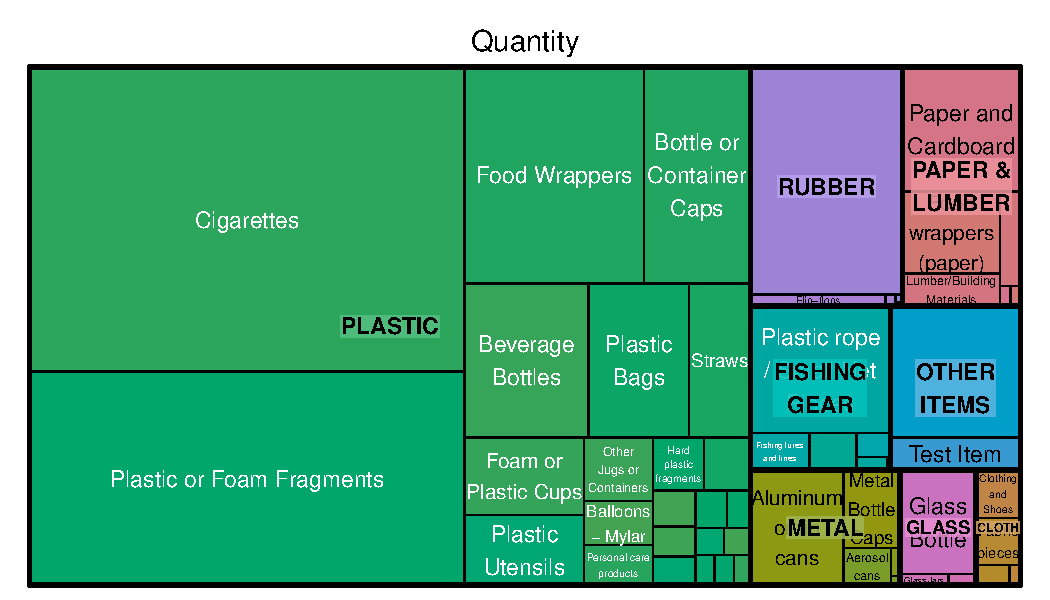
\includegraphics[width=1\linewidth]{figure/unnamed-chunk-12-1} 
\begin{kframe}\begin{alltt}
    \hlcom{#scale_fill_viridis_d(option = "magma")}

\hlcom{#ggsave("plots/pastic_debris_plot.png", width = 40, height = 20, units = "cm")}
\end{alltt}
\end{kframe}
\end{knitrout}
\caption {Debris by categorisation}
\label{figE}
\end {center}
\end {figure}


\begin{knitrout}\small
\definecolor{shadecolor}{rgb}{0.969, 0.969, 0.969}\color{fgcolor}\begin{kframe}
\begin{alltt}
\hlcom{# all cigarette related waste: 1, 4, 6, 22}
\hlcom{# Food related waste: 3, 2,7,9,10, 17, 23, 11}
\hlcom{# Non food related waste: 8, 14, 15, 16, 18, 19, 21, 20}
\hlcom{# Plastic bags and Styrofoam packaging:12, 13}
\hlcom{# Fragments: 5, 23, 24,25}

\hlstd{recategorise} \hlkwb{<-} \hlkwa{function}\hlstd{(}\hlkwc{x}\hlstd{)\{}
  \hlstd{out} \hlkwb{=} \hlstr{""}
  \hlkwa{if}\hlstd{(x} \hlopt \hlkwd{c}\hlstd{(}\hlnum{1}\hlstd{,}\hlnum{4}\hlstd{,}\hlnum{6}\hlstd{,}\hlnum{22}\hlstd{))\{out} \hlkwb{=} \hlstr{"Cigarette related waste"}\hlstd{\}}
  \hlkwa{if}\hlstd{(x} \hlopt \hlkwd{c}\hlstd{(}\hlnum{2}\hlstd{,}\hlnum{3}\hlstd{,}\hlnum{7}\hlstd{,}\hlnum{9}\hlstd{,}\hlnum{10}\hlstd{,}\hlnum{17}\hlstd{,}\hlnum{23}\hlstd{,}\hlnum{11}\hlstd{)) out} \hlkwb{=} \hlstr{"Food related waste"}
  \hlkwa{if}\hlstd{(x} \hlopt \hlkwd{c}\hlstd{(}\hlnum{8}\hlstd{,}\hlnum{14}\hlstd{,}\hlnum{15}\hlstd{,}\hlnum{16}\hlstd{,}\hlnum{18}\hlstd{,}\hlnum{19}\hlstd{,}\hlnum{21}\hlstd{,}\hlnum{20}\hlstd{)) out} \hlkwb{=} \hlstr{"Other"}
  \hlkwa{if}\hlstd{(x} \hlopt \hlkwd{c}\hlstd{(}\hlnum{12}\hlstd{,}\hlnum{13}\hlstd{)) out} \hlkwb{=} \hlstr{"Plastic bags and Styrofoam packaging"}
  \hlkwa{if}\hlstd{(x} \hlopt \hlkwd{c}\hlstd{(}\hlnum{5}\hlstd{,}\hlnum{23}\hlstd{,}\hlnum{24}\hlstd{,}\hlnum{25}\hlstd{)) out} \hlkwb{=} \hlstr{"Fragments"}
  \hlkwa{if}\hlstd{(out} \hlopt{==} \hlstr{""}\hlstd{)} \hlkwd{stop}\hlstd{(}\hlkwd{paste}\hlstd{(}\hlstr{"Error in recategorise:"}\hlstd{, x))}
  \hlkwd{return}\hlstd{(out)}
\hlstd{\}}

\hlstd{plastic_types} \hlkwb{<-} \hlstd{data} \hlopt
  \hlkwd{filter}\hlstd{(`Material Description`} \hlopt{==} \hlstr{"PLASTIC"}\hlstd{)} \hlopt
  \hlkwd{select}\hlstd{(ItemName, ItemID)} \hlopt
  \hlkwd{distinct}\hlstd{()} \hlopt
  \hlkwd{mutate}\hlstd{(}\hlkwc{label} \hlstd{=} \hlnum{1}\hlopt{:}\hlkwd{n}\hlstd{())} \hlopt
  \hlkwd{mutate}\hlstd{(}\hlkwc{category} \hlstd{= purrr}\hlopt{::}\hlkwd{map}\hlstd{(label, recategorise))} \hlopt
  \hlkwd{mutate}\hlstd{(}\hlkwc{category} \hlstd{=} \hlkwd{as_factor}\hlstd{(}\hlkwd{as.character}\hlstd{(category)))} \hlopt
  \hlkwd{select}\hlstd{(ItemID, category)}


\hlstd{plastic} \hlkwb{<-} \hlstd{data} \hlopt
  \hlkwd{filter}\hlstd{(`Material Description`} \hlopt{==} \hlstr{"PLASTIC"}\hlstd{)} \hlopt
  \hlkwd{full_join}\hlstd{(plastic_types,} \hlkwc{by} \hlstd{=} \hlstr{"ItemID"}\hlstd{)}

\hlstd{ordered_levels} \hlkwb{<-} \hlstd{plastic} \hlopt
  \hlkwd{group_by}\hlstd{(category)} \hlopt
  \hlkwd{summarise}\hlstd{(}\hlkwc{totObs} \hlstd{=} \hlkwd{sum}\hlstd{(Quantity))} \hlopt
  \hlkwd{ungroup}\hlstd{()} \hlopt
  \hlkwd{arrange}\hlstd{(}\hlkwd{desc}\hlstd{(totObs))} \hlopt
  \hlkwd{select}\hlstd{(category)} \hlopt
  \hlstd{category}
\hlstd{plastic}\hlopt{$}\hlstd{category} \hlkwb{<-} \hlkwd{factor}\hlstd{(plastic}\hlopt{$}\hlstd{category,} \hlkwc{levels} \hlstd{= ordered_levels)}
\hlkwd{rm}\hlstd{(ordered_levels)}
\end{alltt}
\end{kframe}
\end{knitrout}

\begin{figure}[H]
\begin{center}
\begin{knitrout}\small
\definecolor{shadecolor}{rgb}{0.969, 0.969, 0.969}\color{fgcolor}\begin{kframe}
\begin{alltt}
\hlstd{plastic} \hlopt
  \hlkwd{mutate}\hlstd{(}\hlkwc{month} \hlstd{=} \hlkwd{month}\hlstd{(Time,} \hlkwc{label} \hlstd{=} \hlnum{FALSE}\hlstd{),}
         \hlkwc{year} \hlstd{=} \hlkwd{as.integer}\hlstd{(}\hlkwd{year}\hlstd{(Time)))} \hlopt
  \hlkwd{group_by}\hlstd{(month, year, category)} \hlopt
  \hlkwd{summarise}\hlstd{(}\hlkwc{`Total Quantity`} \hlstd{=} \hlkwd{sum}\hlstd{(Quantity))} \hlopt
  \hlkwd{ggplot}\hlstd{(}\hlkwd{aes}\hlstd{(}\hlkwc{x} \hlstd{= month,} \hlkwc{y} \hlstd{= `Total Quantity`,} \hlkwc{fill} \hlstd{= category))} \hlopt{+}
    \hlkwd{geom_col}\hlstd{(}\hlkwc{colour} \hlstd{=} \hlstr{"black"}\hlstd{,} \hlkwc{size} \hlstd{=} \hlnum{0.2}\hlstd{,} \hlkwc{position} \hlstd{=} \hlstr{"fill"}\hlstd{)} \hlopt{+}
    \hlkwd{facet_wrap}\hlstd{(}\hlopt{~}\hlstd{year,} \hlkwc{nrow} \hlstd{=} \hlnum{2}\hlstd{)} \hlopt{+}
    \hlkwd{scale_fill_viridis}\hlstd{(}\hlkwc{discrete} \hlstd{=} \hlnum{TRUE}\hlstd{,} \hlkwc{option} \hlstd{=} \hlstr{"plasma"}\hlstd{)} \hlopt{+}
    \hlkwd{xlab}\hlstd{(}\hlstr{"Month"}\hlstd{)} \hlopt{+}
    \hlkwd{ylab}\hlstd{(}\hlstr{"Proportion of Items"}\hlstd{)} \hlopt{+}
    \hlkwd{ggtitle}\hlstd{(}\hlstr{"Rel. frequencies of observed plastic waste by category"}\hlstd{)} \hlopt{+}
    \hlkwd{scale_x_continuous}\hlstd{(}\hlkwc{breaks} \hlstd{=} \hlnum{1}\hlopt{:}\hlnum{12}\hlstd{)} \hlopt{+}
    \hlkwd{theme}\hlstd{(}\hlkwc{panel.grid.major.x} \hlstd{=} \hlkwd{element_blank}\hlstd{(),}
          \hlkwc{panel.grid.minor.x} \hlstd{=} \hlkwd{element_blank}\hlstd{(),}
          \hlkwc{legend.position} \hlstd{=} \hlstr{"bottom"}\hlstd{,}
          \hlkwc{legend.text}\hlstd{=}\hlkwd{element_text}\hlstd{(}\hlkwc{size}\hlstd{=}\hlnum{5}\hlstd{))} \hlopt{+}
    \hlkwd{guides}\hlstd{(}\hlkwc{fill}\hlstd{=}\hlkwd{guide_legend}\hlstd{(}\hlkwc{title}\hlstd{=}\hlstr{"Category"}\hlstd{))}
\end{alltt}
\end{kframe}
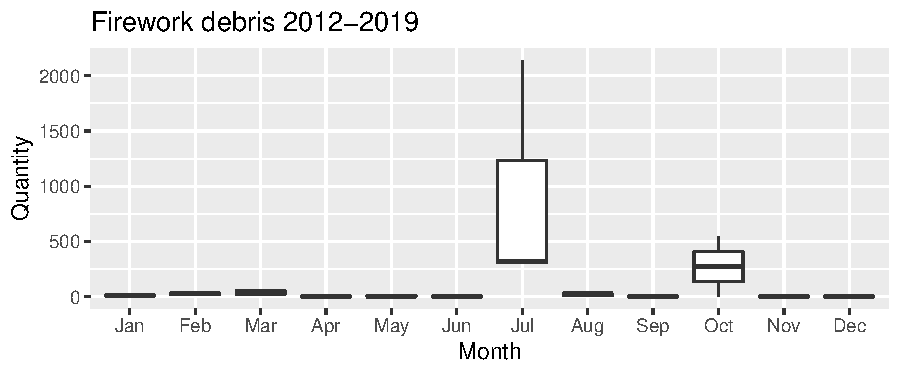
\includegraphics[width=1\linewidth]{figure/unnamed-chunk-14-1} 
\begin{kframe}\begin{alltt}
\hlcom{#ggsave("plots/pastic_debris_plot_recategorised.png", width = 40, height = 20, units = "cm")}
\end{alltt}
\end{kframe}
\end{knitrout}
\caption {Recategorisation by year. Colour scale ordered by ranking of total observed quantity.}
\label{figB}
\end {center}
\end {figure}


















\pagebreak
\section{Exploration}



\subsection{Proportion Trends}
% The key variable in this section is TIME (Years, Months)
After cleaning and recategorisation of the data, it was analysed to determine how pollutant proportions change over time. 1. using the CCI categories, 2. using the original subcategories.\\

Per the data, we see an increase in debris observed over time. Caution must be exercised in interpreting this information, as this increase may be reflective indeed of increased pollution levels, but it could also be because the citizen science project has gained popularity and more organisations and individual observations.

\begin{figure}[H] 
\begin{center}
\begin{knitrout}\small
\definecolor{shadecolor}{rgb}{0.969, 0.969, 0.969}\color{fgcolor}\begin{kframe}
\begin{alltt}
\hlcom{#Linechart quantity of debris per year}
\hlstd{data} \hlopt
  \hlkwd{mutate}\hlstd{(}\hlkwc{year} \hlstd{=} \hlkwd{year}\hlstd{(Time))} \hlopt
  \hlkwd{group_by}\hlstd{(year)} \hlopt
  \hlkwd{summarise}\hlstd{(}\hlkwc{quan} \hlstd{=} \hlkwd{sum}\hlstd{(Quantity))} \hlopt
  \hlkwd{ggplot}\hlstd{(}\hlkwd{aes}\hlstd{(}\hlkwc{x} \hlstd{= year,} \hlkwc{y} \hlstd{= quan))} \hlopt{+}
    \hlkwd{geom_col}\hlstd{()} \hlopt{+}
    \hlkwd{scale_x_continuous}\hlstd{(}\hlkwc{breaks} \hlstd{=} \hlnum{2012}\hlopt{:}\hlnum{2019}\hlstd{)} \hlopt{+}
    \hlkwd{xlab}\hlstd{(}\hlstr{"Year"}\hlstd{)} \hlopt{+}
    \hlkwd{ylab}\hlstd{(}\hlstr{"Quantity"}\hlstd{)} \hlopt{+}
    \hlkwd{ggtitle}\hlstd{(}\hlstr{"Quantity of debris per year"}\hlstd{)} \hlopt{+}
    \hlkwd{theme}\hlstd{(}\hlkwc{panel.grid.major.x} \hlstd{=} \hlkwd{element_blank}\hlstd{(),}
          \hlkwc{panel.grid.minor.x} \hlstd{=} \hlkwd{element_blank}\hlstd{())} \hlopt{+}
    \hlkwd{scale_y_continuous}\hlstd{(}\hlkwc{labels} \hlstd{= scales}\hlopt{::}\hlkwd{label_number_si}\hlstd{(}\hlkwc{accuracy} \hlstd{=} \hlnum{1}\hlstd{))}
\end{alltt}
\end{kframe}
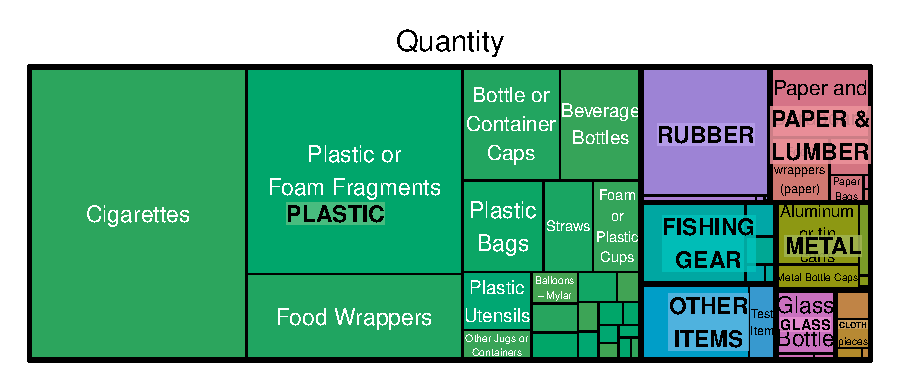
\includegraphics[width=1\linewidth]{figure/unnamed-chunk-15-1} 
\begin{kframe}\begin{alltt}
\hlcom{#ggsave("plots/observations.png")}
\end{alltt}
\end{kframe}
\end{knitrout}
\caption {Trend of debris observered}
\label{figD}
\end {center}
\end {figure}


\hl{insert: count of unique observations, maybe grouped by average number of observation entries per day? - we want to try and identify increase in user activity}\\
As we see in the chart above, an increase in the number of average observations per day lends support to the theory that the increase in observations is factored by increase in citizen science monitoring activity. That's not to say pollution hasn't also increased in this period, but it would be inaccurate to not account for the increase in monitoring activity.\\




\hl{insert: proportion changes of MATERIAL TYPES over years. Line or column. We want to prove that plastic is the dominant pollutant and possibly the only increasing one }
Analysis of the poportions of pollutant materials suggests that not only is plastic the dominant marine pollutant material, its proportion of total debris is increasingly observed year on year. This could be due to an increase in new plastic pollution entering marine environments from source, not helped by the fact it is durable and doesn't decompose, as discussed in the introduction of this report, or that the other pollutant materials are decreasing. Of all the pollutant materials listed here - plastic is the most longlife \hl{can we support this statement?}. This analysis therefore is in agreement with the studies discussed in section 2 of this report that plastic is indeed the biggest problem in marine pollution. 




\begin{figure}[H] 
\begin{center}
\begin{knitrout}\small
\definecolor{shadecolor}{rgb}{0.969, 0.969, 0.969}\color{fgcolor}\begin{kframe}
\begin{alltt}
\hlcom{#Histogram of observations: Total v Plastic}
\hlstd{data} \hlopt
  \hlkwd{mutate}\hlstd{(}\hlkwc{Type} \hlstd{=} \hlkwd{if_else}\hlstd{(`Material Description`} \hlopt{==} \hlstr{"PLASTIC"}\hlstd{,} \hlstr{"Plastic"}\hlstd{,} \hlstr{"Other"}\hlstd{),}
         \hlkwc{months} \hlstd{=} \hlkwd{floor_date}\hlstd{(Time,} \hlstr{'month'}\hlstd{))} \hlopt
  \hlkwd{group_by}\hlstd{(months, Type)} \hlopt
  \hlkwd{summarize}\hlstd{(}\hlkwc{`Number of observations`} \hlstd{=} \hlkwd{n}\hlstd{())} \hlopt
  \hlkwd{ggplot}\hlstd{(}\hlkwd{aes}\hlstd{(}\hlkwc{x} \hlstd{= months,} \hlkwc{y} \hlstd{= `Number of observations`))} \hlopt{+}
    \hlkwd{geom_area}\hlstd{(}\hlkwd{aes}\hlstd{(}\hlkwc{fill} \hlstd{= Type))} \hlopt{+}
    \hlkwd{theme}\hlstd{(}\hlkwc{legend.position} \hlstd{=} \hlstr{"bottom"}\hlstd{)}
\end{alltt}
\end{kframe}
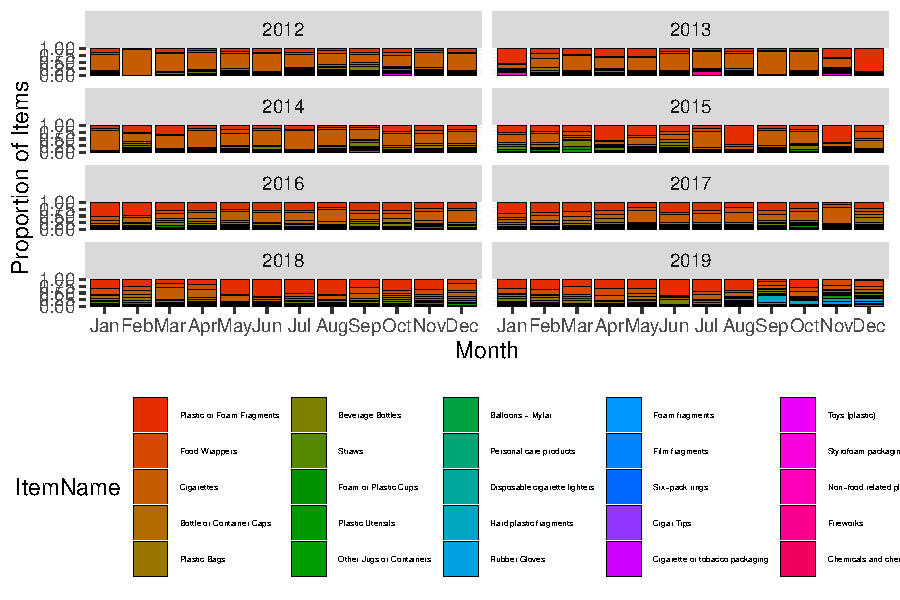
\includegraphics[width=1\linewidth]{figure/unnamed-chunk-16-1} 
\begin{kframe}\begin{alltt}
  \hlcom{# ggplot() +}
  \hlcom{# geom_histogram(aes(x = Time))}
\end{alltt}
\end{kframe}
\end{knitrout}
\caption {Observations of plastic debris v all debris}
\label{figF}
\end {center}
\end {figure}
\hl{minor edit: can we take away the area fill but keep the coloured lines?}\\

\hl{insert: line chart of just the \% plastic over years}

When we consider the charts above, we can determine that it is not only the plastic proportion of total pollutant materials that increases, but it's total observation counts too (not quanitities). This means that even as more debris are observed, plastics remain a consistently common feature of the observed derbis.\\

In this chart we also see peaks and troughs in the number of observations - this is indicative of an increase in user activity. Seeing the peak in 2013 - that's not to say pollution suddenly increased in one period and disappeared, but monitoring activity spiked in that period. \hl{do we know why?} We see more of these spikes in 2017, 2018 and 2019 but generally it is an increasing trend in monitoring activity.\\


\hl{insert: proportion changes of RECATEGORISED plastic over years. stacked lines or columns}
When considering the subcategories within plastic we see..... \hl{can we link this to decreasing cigarettes?}

\hl{insert: table of \% change in ItemNames 2012 to 2019. return top 10 or 15 ABSOLUTE value changes. If you really want to do this properly you'll take the averaged change in \% year on year and compare it to the end-to-end \% change.}

An interesting observation was that as Old pollutants fall away (cigarette butts) but new ones are introduced. Cigarette butts proportions and raw counts decrease over time which is possibly indicative of less people smoking, or moving to vaping \hl{source this, or don't bother?}\\


\subsection {Distribution of observed debris:}

MaterialQuantities\\

\begin{figure}[H] 
\begin{center}
\begin{knitrout}\small
\definecolor{shadecolor}{rgb}{0.969, 0.969, 0.969}\color{fgcolor}\begin{kframe}
\begin{alltt}
\hlstd{data} \hlopt \hlkwd{select}\hlstd{(Quantity,Description,`Material Description`)} \hlopt
  \hlkwd{group_by}\hlstd{(`Material Description`)} \hlopt
  \hlkwd{summarise}\hlstd{(}\hlkwc{Quantity} \hlstd{=} \hlkwd{sum}\hlstd{(Quantity))} \hlopt

  \hlkwd{ggplot}\hlstd{(}\hlkwd{aes}\hlstd{(}\hlkwc{x} \hlstd{=} \hlkwd{reorder}\hlstd{(`Material Description`, Quantity),} \hlkwc{y} \hlstd{= Quantity))} \hlopt{+}
    \hlkwd{geom_col}\hlstd{()} \hlopt{+}
    \hlkwd{ylab}\hlstd{(}\hlstr{"Total recorded quantity"}\hlstd{)} \hlopt{+}
    \hlkwd{xlab}\hlstd{(}\hlstr{"Material class"}\hlstd{)} \hlopt{+}
    \hlkwd{coord_flip}\hlstd{()}
\end{alltt}
\end{kframe}
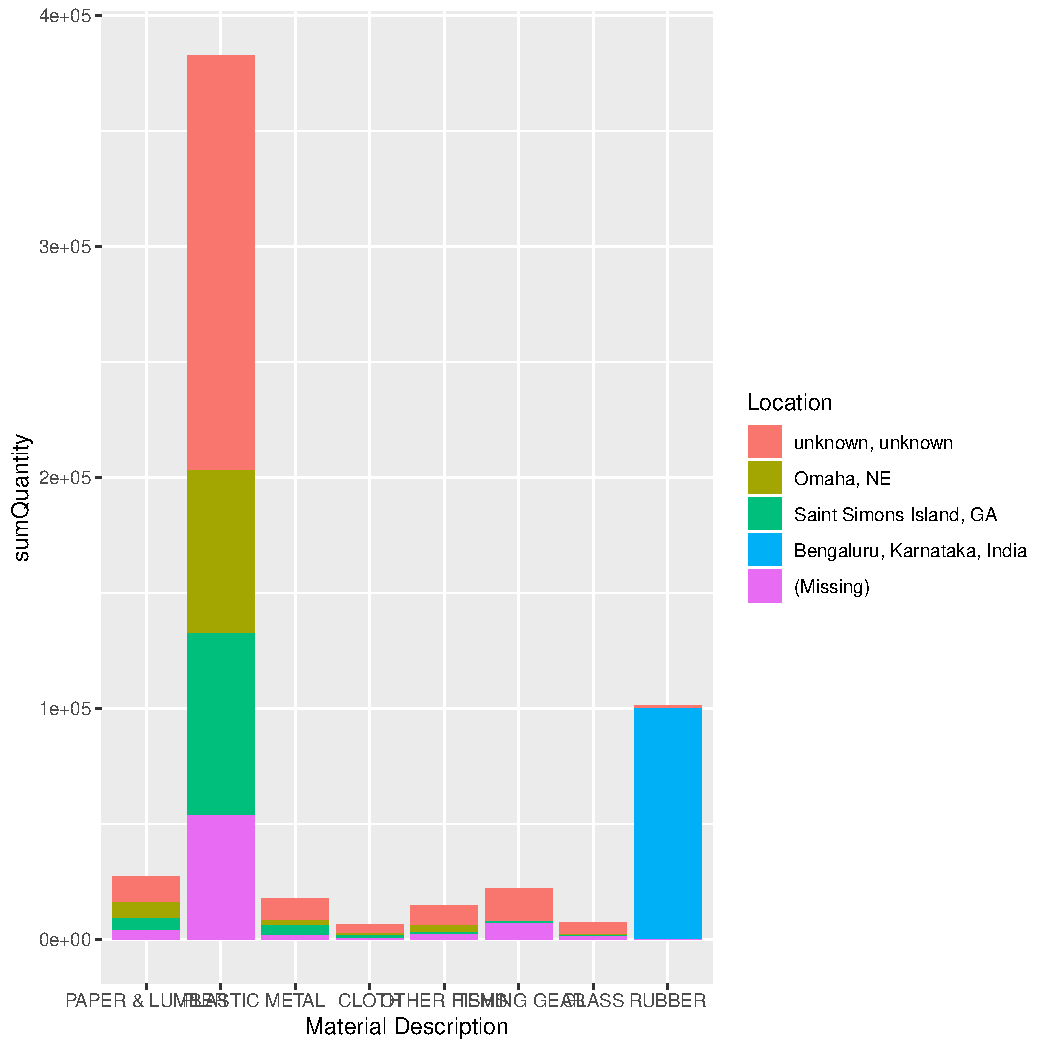
\includegraphics[width=1\linewidth]{figure/unnamed-chunk-17-1} 

\end{knitrout}
\caption {Material Quantities}
\label{figC}
\end {center}
\end {figure}

So the most populated material class is Plastic. Note that this does not necessarily mean that plastic is the largest quantity of debris, just that the individual number of items categorised is largest.

A tree map of material quantities:
\begin{figure}[H] 
\begin{center}
\begin{knitrout}\small
\definecolor{shadecolor}{rgb}{0.969, 0.969, 0.969}\color{fgcolor}\begin{kframe}
\begin{alltt}
\hlcom{#treemap of debris categories}
\hlcom{#png("plots/treemap.png")}
\hlstd{data} \hlopt
  \hlkwd{select}\hlstd{(`Material Description`, ItemName, Quantity)} \hlopt
  \hlkwd{group_by}\hlstd{(`Material Description`, ItemName)} \hlopt
  \hlkwd{summarise}\hlstd{(}\hlkwc{Quantity} \hlstd{=} \hlkwd{sum}\hlstd{(Quantity))} \hlopt
  \hlkwd{treemap}\hlstd{(}\hlkwc{index} \hlstd{=} \hlkwd{c}\hlstd{(}\hlstr{"Material Description"}\hlstd{,} \hlstr{"ItemName"}\hlstd{),}
          \hlkwc{vSize} \hlstd{=} \hlstr{"Quantity"}\hlstd{,} \hlkwc{draw} \hlstd{=} \hlnum{TRUE}\hlstd{)} \hlkwb{->} \hlstd{tm}
\end{alltt}
\end{kframe}
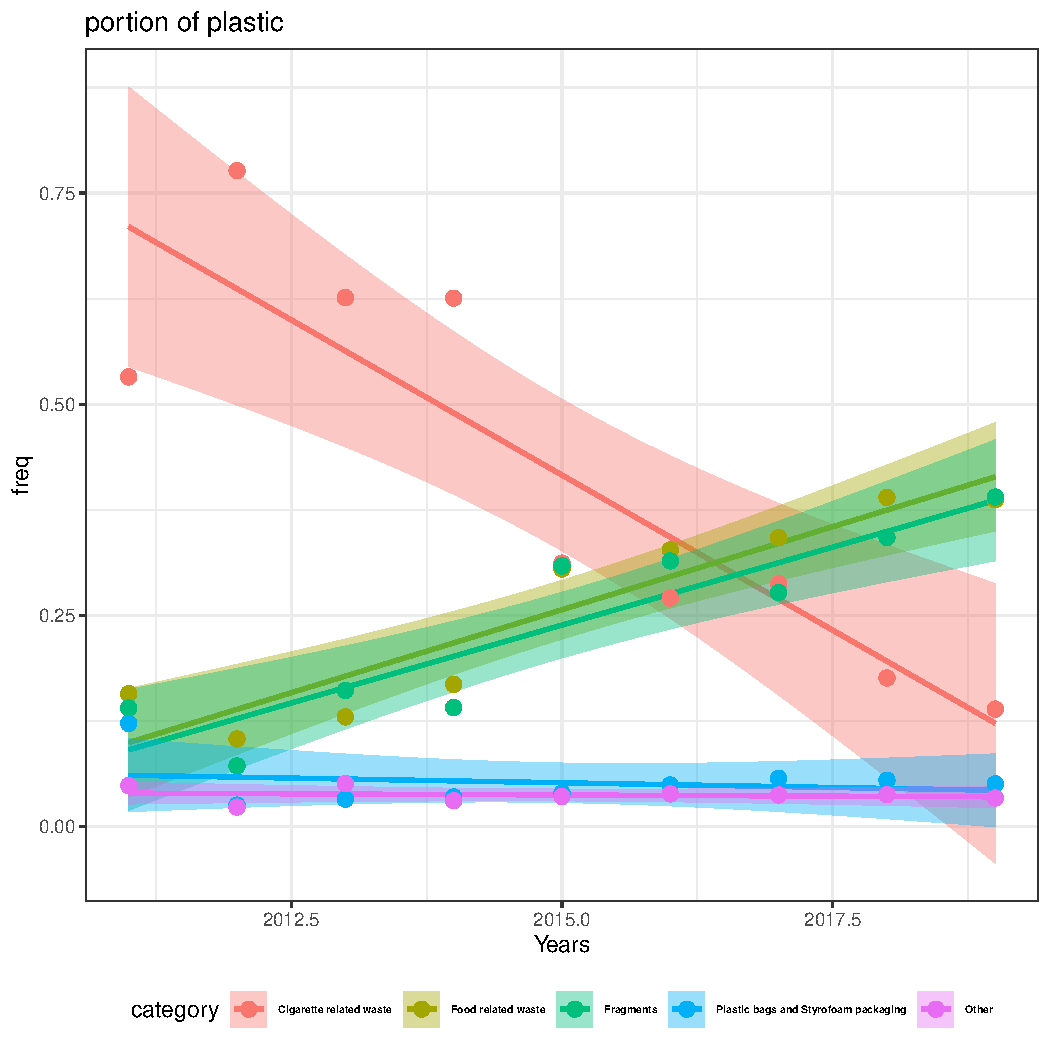
\includegraphics[width=1\linewidth]{figure/unnamed-chunk-18-1} 
\begin{kframe}\begin{alltt}
\hlcom{#tm}
\hlcom{#dev.off()}
\hlcom{#save.image(file = "plots/treemap.png")}
\end{alltt}
\end{kframe}
\end{knitrout}
\caption {Debris categorisation}
\label{figI}
\end {center}
\end {figure}

Cigarettes are the most common item recorded as seen in. %Figure~\ref{figI}
Perhaps some of the debris is not actually from the sea, but rather from people littering by the coastline? Does debris littered on the coastline end up in the oceans?

\hl{This is a great chart, but not the best to support the statement that cigarettes is most popular - a column or bar chart here will be much better (area charts are not as effective as charts you can level-compare), potentially use proportions or data labels to further drive the point that it IS the largest. Treemap suggest moving back into pre-processing section.}


\begin{figure}[H] 
\begin{center}
\begin{knitrout}\small
\definecolor{shadecolor}{rgb}{0.969, 0.969, 0.969}\color{fgcolor}\begin{kframe}
\begin{alltt}
\hlcom{#bar of debris categories}
\hlstd{data} \hlopt
  \hlkwd{select}\hlstd{(`Material Description`, ItemName, Quantity)} \hlopt
  \hlkwd{group_by}\hlstd{(`Material Description`, ItemName)} \hlopt
  \hlkwd{summarise}\hlstd{(}\hlkwc{Quantity} \hlstd{=} \hlkwd{sum}\hlstd{(Quantity))} \hlopt
  \hlkwd{ggplot}\hlstd{(}\hlkwd{aes}\hlstd{(}\hlkwc{x}\hlstd{=}\hlkwd{reorder}\hlstd{(`ItemName`,} \hlopt{-}\hlstd{Quantity),} \hlkwc{y}\hlstd{=Quantity,} \hlkwc{fill}\hlstd{=`Material Description`))} \hlopt{+}
  \hlkwd{geom_bar}\hlstd{(}\hlkwc{stat}\hlstd{=}\hlstr{"identity"}\hlstd{)} \hlopt{+}
  \hlkwd{ggtitle}\hlstd{(}\hlstr{"Debris Categorisation"}\hlstd{)} \hlopt{+}
  \hlkwd{xlab}\hlstd{(}\hlstr{"Debris"}\hlstd{)} \hlopt{+}
  \hlkwd{ylab}\hlstd{(}\hlstr{""}\hlstd{)} \hlopt{+}
  \hlcom{#coord_flip() +}
  \hlkwd{theme}\hlstd{(}\hlkwc{text} \hlstd{=} \hlkwd{element_text}\hlstd{(}\hlkwc{size}\hlstd{=}\hlnum{8}\hlstd{),}
        \hlkwc{axis.text.x}\hlstd{=}\hlkwd{element_text}\hlstd{(}\hlkwc{angle}\hlstd{=}\hlnum{90}\hlstd{,} \hlkwc{hjust}\hlstd{=}\hlnum{1}\hlstd{),}
        \hlkwc{plot.title} \hlstd{=} \hlkwd{element_text}\hlstd{(}\hlkwc{size}\hlstd{=}\hlnum{10}\hlstd{),}
        \hlkwc{legend.text}\hlstd{=}\hlkwd{element_text}\hlstd{(}\hlkwc{size}\hlstd{=}\hlnum{5}\hlstd{),}
        \hlkwc{legend.position} \hlstd{=} \hlstr{"bottom"}\hlstd{)}
\end{alltt}
\end{kframe}
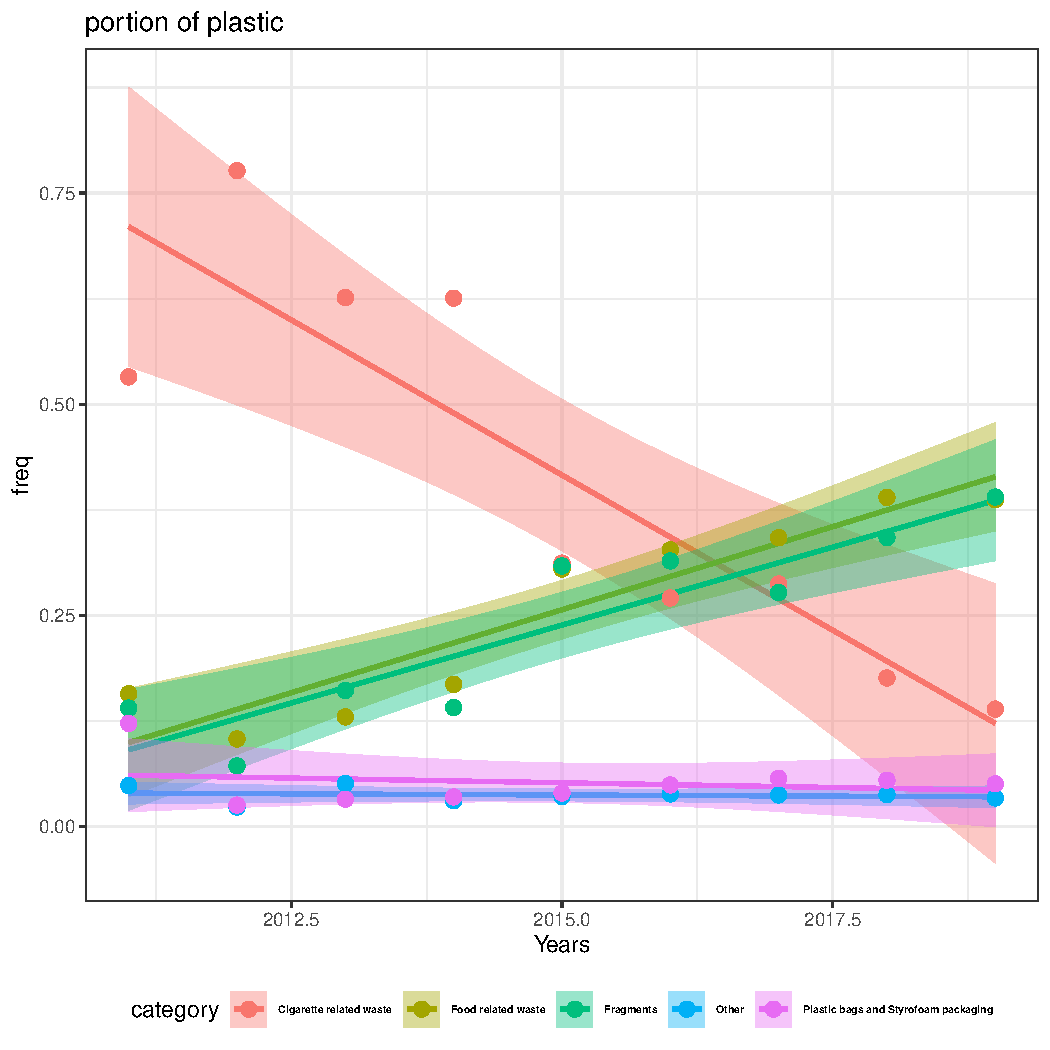
\includegraphics[width=1\linewidth]{figure/unnamed-chunk-19-1} 
\begin{kframe}\begin{alltt}
  \hlcom{#treemap(index = c("Material Description", "ItemName"),}
  \hlcom{#        vSize = "Quantity", draw = TRUE) -> tm}
\end{alltt}
\end{kframe}
\end{knitrout}
\caption {Debris categorisation}
\label{figI2}
\end {center}
\end {figure}

\hl{maybe make this top 10 or 15 items.}


\pagebreak
\subsection{Event-Driven Pollution}

Fireworks found in July and North-America only: possibly 4th July celebrations\\
4th July and Firework link? (Karen's Idea)\\

\begin{figure}[H] 
\begin{center}
\begin{knitrout}\small
\definecolor{shadecolor}{rgb}{0.969, 0.969, 0.969}\color{fgcolor}\begin{kframe}
\begin{alltt}
\hlcom{#Boxplot of fireworks distribution by month (across all years)}
\hlstd{data} \hlopt
  \hlkwd{filter}\hlstd{(`Material Description`} \hlopt{==} \hlstr{"PLASTIC"}\hlstd{,}
         \hlstd{ItemName} \hlopt \hlkwd{c}\hlstd{(}\hlstr{"Fireworks"}\hlstd{),}
         \hlkwd{year}\hlstd{(Time)} \hlopt{>=} \hlnum{2012}\hlstd{,} \hlkwd{year}\hlstd{(Time)} \hlopt{<=} \hlnum{2019}\hlstd{)} \hlopt
  \hlkwd{mutate}\hlstd{(}\hlkwc{month} \hlstd{=} \hlkwd{month}\hlstd{(Time,} \hlkwc{label} \hlstd{=} \hlnum{TRUE}\hlstd{),}
         \hlkwc{year} \hlstd{=} \hlkwd{as.integer}\hlstd{(}\hlkwd{year}\hlstd{(Time)))} \hlopt
  \hlkwd{group_by}\hlstd{(month, year)} \hlopt
  \hlkwd{summarise}\hlstd{(}\hlkwc{quantity} \hlstd{=} \hlkwd{sum}\hlstd{(Quantity))} \hlopt
  \hlkwd{ggplot}\hlstd{()} \hlopt{+}
    \hlkwd{geom_boxplot}\hlstd{(}\hlkwd{aes}\hlstd{(}\hlkwc{x} \hlstd{= month,} \hlkwc{y} \hlstd{= quantity))} \hlopt{+}
    \hlkwd{xlab}\hlstd{(}\hlstr{"Month"}\hlstd{)} \hlopt{+}
    \hlkwd{ylab}\hlstd{(}\hlstr{"Quantity"}\hlstd{)} \hlopt{+}
    \hlkwd{ggtitle}\hlstd{(}\hlstr{"Firework debris 2012-2019"}\hlstd{)}
\end{alltt}
\end{kframe}
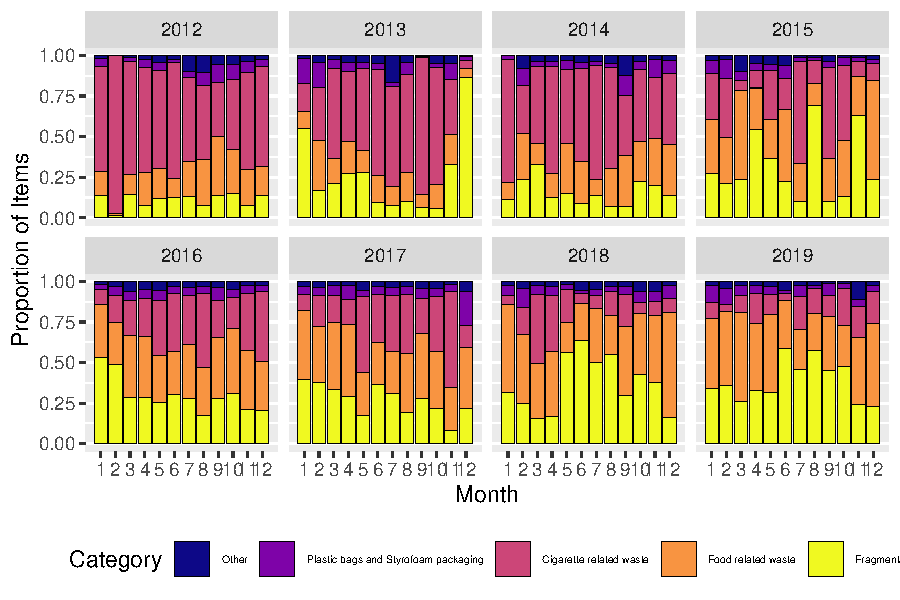
\includegraphics[width=1\linewidth]{figure/unnamed-chunk-20-1} 
\begin{kframe}\begin{alltt}
\hlcom{#ggsave("plots/fireworks.png")}
\end{alltt}
\end{kframe}
\end{knitrout}

\caption {Boxplot of fireworks distribution by month, across all years}
\label{figA}
\end {center}
\end {figure}


\pagebreak
\subsection{Location-Driven Pollution}

Rubber found in Indoneasia only: possibly a recording bias.\\

Certain classes are found in certain regions only: not because they don't exist elsewhere but because of recording bias focus in those areas\\

We have locational data, so lets check for any geographical observation bias.
\begin{knitrout}\small
\definecolor{shadecolor}{rgb}{0.969, 0.969, 0.969}\color{fgcolor}\begin{kframe}
\begin{alltt}
\hlstd{world} \hlkwb{<-} \hlkwd{map_data}\hlstd{(}\hlstr{"world"}\hlstd{)}
\hlstd{data} \hlopt
  \hlkwd{select}\hlstd{(Latitude, Longitude, Quantity, Location, `Material Description`)} \hlopt
  \hlkwd{ggplot}\hlstd{()} \hlopt{+}
    \hlkwd{geom_polygon}\hlstd{(}\hlkwc{data} \hlstd{=} \hlkwd{map_data}\hlstd{(}\hlstr{"world"}\hlstd{),} \hlkwd{aes}\hlstd{(}\hlkwc{x} \hlstd{= long,} \hlkwc{y} \hlstd{= lat,} \hlkwc{group} \hlstd{= group),} \hlkwc{fill} \hlstd{=} \hlstr{"grey"}\hlstd{,} \hlkwc{alpha} \hlstd{=} \hlnum{0.5}\hlstd{)} \hlopt{+}
    \hlkwd{geom_hex}\hlstd{(}\hlkwd{aes}\hlstd{(}\hlkwc{x} \hlstd{= Longitude,} \hlkwc{y} \hlstd{= Latitude),} \hlkwc{bins} \hlstd{=} \hlnum{50}\hlstd{)} \hlopt{+}
    \hlkwd{scale_fill_viridis}\hlstd{(}\hlkwc{trans} \hlstd{=} \hlstr{"log"}\hlstd{,} \hlkwc{breaks} \hlstd{=} \hlkwd{c}\hlstd{(}\hlnum{5}\hlstd{,} \hlnum{50}\hlstd{,} \hlnum{500}\hlstd{,} \hlnum{5000}\hlstd{,} \hlnum{50000}\hlstd{))} \hlopt{+}
    \hlkwd{theme_void}\hlstd{()} \hlopt{+}
    \hlkwd{guides}\hlstd{(}\hlkwc{fill}\hlstd{=}\hlkwd{guide_legend}\hlstd{(}\hlkwc{title}\hlstd{=}\hlstr{"Observations"}\hlstd{))}
\end{alltt}
\end{kframe}
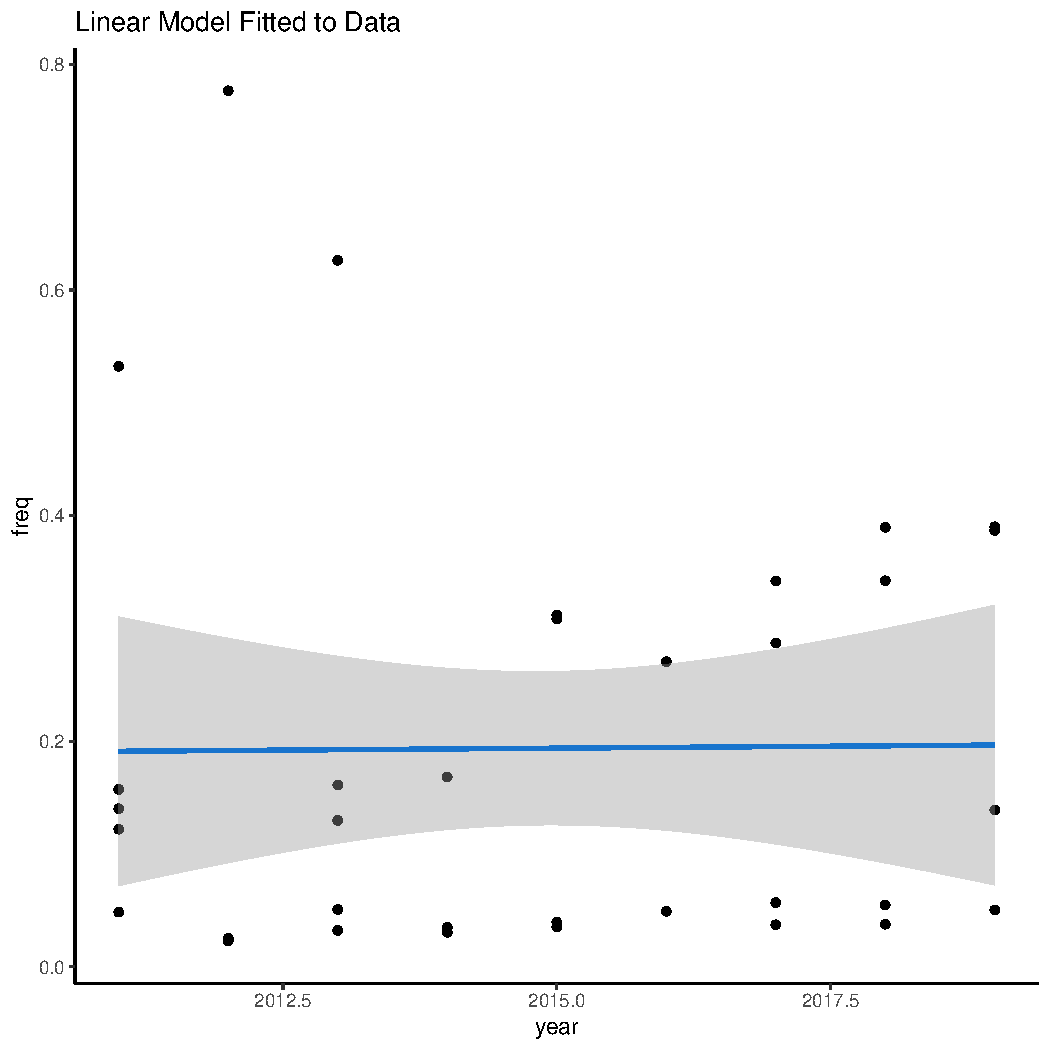
\includegraphics[width=1\linewidth]{figure/unnamed-chunk-21-1} 
\begin{kframe}\begin{alltt}
\hlcom{#ggsave("plots/map.png", width = 20, height = 10, units = "cm")}
\end{alltt}
\end{kframe}
\end{knitrout}

We need to know how reliable the location data is. I'm going to filter for "united kingdom" in the location field and plot the raw coordinates.\\

\begin{figure}[H] 
\begin{center}

\caption {Longitude and Latitude discrepancies}
\label{figJ}
\end {center}
\end {figure}


Questions\\
Distribution of plastic by location.\\
Are the distributions of plastic fairly constant for the locations with the most observations?\\
\begin{figure}[H] 
\begin{center}
\begin{knitrout}\small
\definecolor{shadecolor}{rgb}{0.969, 0.969, 0.969}\color{fgcolor}\begin{kframe}
\begin{alltt}
\hlcom{#columnchart of debris locations}
\hlstd{topLocations} \hlkwb{<-} \hlstd{data} \hlopt
  \hlkwd{group_by}\hlstd{(Location)} \hlopt
  \hlkwd{summarise}\hlstd{(}\hlkwc{sumQuantity} \hlstd{=} \hlkwd{sum}\hlstd{(Quantity))} \hlopt
  \hlkwd{arrange}\hlstd{(}\hlkwd{desc}\hlstd{(sumQuantity))} \hlopt
  \hlkwd{top_n}\hlstd{(}\hlnum{5}\hlstd{,sumQuantity)}

\hlstd{data} \hlopt
  \hlkwd{filter}\hlstd{(Location} \hlopt \hlstd{topLocations}\hlopt{$}\hlstd{Location)} \hlopt
  \hlkwd{group_by}\hlstd{(Location, `Material Description`)} \hlopt
  \hlkwd{summarise}\hlstd{(}\hlkwc{sumQuantity} \hlstd{=} \hlkwd{sum}\hlstd{(Quantity))} \hlopt
  \hlkwd{arrange}\hlstd{(}\hlkwd{desc}\hlstd{(sumQuantity))} \hlopt
  \hlkwd{ggplot}\hlstd{(}\hlkwd{aes}\hlstd{(}\hlkwc{x} \hlstd{= `Material Description`,} \hlkwc{y} \hlstd{= sumQuantity,} \hlkwc{fill} \hlstd{= Location))} \hlopt{+}
    \hlkwd{geom_col}\hlstd{()} \hlopt{+} \hlkwd{theme}\hlstd{(}\hlkwc{legend.position} \hlstd{=} \hlstr{'top'}\hlstd{)}
\end{alltt}
\end{kframe}
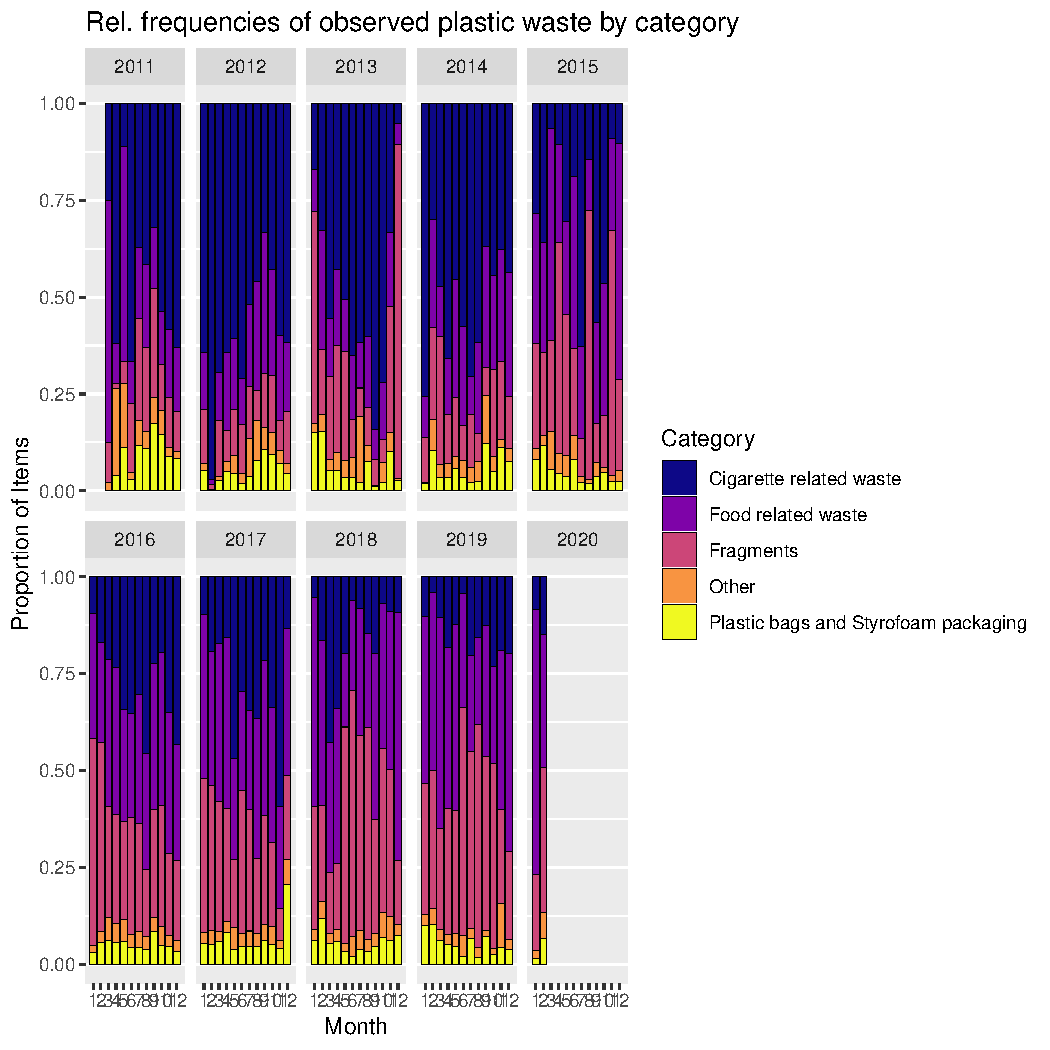
\includegraphics[width=1\linewidth]{figure/unnamed-chunk-23-1} 

\end{knitrout}
\caption {Debris by location}
\label{figG}
\end {center}
\end {figure}
We see that the Location "unknown" has the most plastic... note that this is distinct from "(Missing)", which was our original NA values. Maybe we should merge these.

\pagebreak
\subsection{Item Pairing} 

(e.g. are 6-pack beer rings observed at the same time as fireworks? )
\hl{are we going to explore this one?}



















\pagebreak
\section{Predictive Modelling}
Given the variability of plastic pollution trends given event-driven and location-driven pollution as explored earlier in this report, the authors of this report built a model to predict the proportion of plastics given Month and Location. This would give more accurate predictions as opposed to a simple linear model accomodating such time factored

\subsection{Description of Model}

\begin{knitrout}\small
\definecolor{shadecolor}{rgb}{0.969, 0.969, 0.969}\color{fgcolor}\begin{kframe}
\begin{alltt}
\hlstd{plasticN} \hlkwb{<-} \hlstd{plastic} \hlopt
  \hlkwd{mutate}\hlstd{(}\hlkwc{month} \hlstd{=} \hlkwd{month}\hlstd{(Time,} \hlkwc{label} \hlstd{=} \hlnum{FALSE}\hlstd{),} \hlkwc{year} \hlstd{=} \hlkwd{as.integer}\hlstd{(}\hlkwd{year}\hlstd{(Time)))} \hlopt
  \hlkwd{filter}\hlstd{(year} \hlopt{>} \hlnum{2010}\hlstd{)} \hlopt
  \hlkwd{group_by}\hlstd{(year, category, month)} \hlopt
  \hlkwd{summarise}\hlstd{(}\hlkwc{`Total Quantity`} \hlstd{=} \hlkwd{sum}\hlstd{(Quantity))}

\hlcom{####}


\hlstd{df11N} \hlkwb{<-} \hlstd{plasticN}  \hlopt
  \hlkwd{filter}\hlstd{(year} \hlopt{==} \hlnum{2011}\hlstd{)} \hlopt
  \hlkwd{group_by}\hlstd{(year, month)} \hlopt
  \hlkwd{mutate}\hlstd{(}\hlkwc{freq} \hlstd{= `Total Quantity`} \hlopt{/} \hlkwd{sum}\hlstd{(`Total Quantity`))}

\hlstd{df12N} \hlkwb{<-} \hlstd{plasticN}  \hlopt
  \hlkwd{filter}\hlstd{(year} \hlopt{==} \hlnum{2012}\hlstd{)} \hlopt
  \hlkwd{group_by}\hlstd{(year, month)} \hlopt
  \hlkwd{mutate}\hlstd{(}\hlkwc{freq} \hlstd{= `Total Quantity`} \hlopt{/} \hlkwd{sum}\hlstd{(`Total Quantity`))}


\hlstd{df13N} \hlkwb{<-} \hlstd{plasticN}  \hlopt
  \hlkwd{filter}\hlstd{(year} \hlopt{==} \hlnum{2013}\hlstd{)} \hlopt
  \hlkwd{group_by}\hlstd{(year, month)} \hlopt
  \hlkwd{mutate}\hlstd{(}\hlkwc{freq} \hlstd{= `Total Quantity`} \hlopt{/} \hlkwd{sum}\hlstd{(`Total Quantity`))}


\hlstd{df14N} \hlkwb{<-} \hlstd{plasticN}  \hlopt
  \hlkwd{filter}\hlstd{(year} \hlopt{==} \hlnum{2014}\hlstd{)} \hlopt
  \hlkwd{group_by}\hlstd{(year, month)} \hlopt
  \hlkwd{mutate}\hlstd{(}\hlkwc{freq} \hlstd{= `Total Quantity`} \hlopt{/} \hlkwd{sum}\hlstd{(`Total Quantity`))}

\hlstd{df15N} \hlkwb{<-} \hlstd{plasticN}  \hlopt
  \hlkwd{filter}\hlstd{(year} \hlopt{==} \hlnum{2015}\hlstd{)} \hlopt
  \hlkwd{group_by}\hlstd{(year, month)} \hlopt
  \hlkwd{mutate}\hlstd{(}\hlkwc{freq} \hlstd{= `Total Quantity`} \hlopt{/} \hlkwd{sum}\hlstd{(`Total Quantity`))}


\hlstd{df16N} \hlkwb{<-} \hlstd{plasticN}  \hlopt
  \hlkwd{filter}\hlstd{(year} \hlopt{==} \hlnum{2016}\hlstd{)} \hlopt
  \hlkwd{group_by}\hlstd{(year, month)} \hlopt
  \hlkwd{mutate}\hlstd{(}\hlkwc{freq} \hlstd{= `Total Quantity`} \hlopt{/} \hlkwd{sum}\hlstd{(`Total Quantity`))}



\hlstd{df17N} \hlkwb{<-} \hlstd{plasticN}  \hlopt
  \hlkwd{filter}\hlstd{(year} \hlopt{==} \hlnum{2017}\hlstd{)} \hlopt
  \hlkwd{group_by}\hlstd{(year, month)} \hlopt
  \hlkwd{mutate}\hlstd{(}\hlkwc{freq} \hlstd{= `Total Quantity`} \hlopt{/} \hlkwd{sum}\hlstd{(`Total Quantity`))}


\hlstd{df18N} \hlkwb{<-} \hlstd{plasticN}  \hlopt
  \hlkwd{filter}\hlstd{(year} \hlopt{==} \hlnum{2018}\hlstd{)} \hlopt
  \hlkwd{group_by}\hlstd{(year, month)} \hlopt
  \hlkwd{mutate}\hlstd{(}\hlkwc{freq} \hlstd{= `Total Quantity`} \hlopt{/} \hlkwd{sum}\hlstd{(`Total Quantity`))}

\hlstd{df19N} \hlkwb{<-} \hlstd{plasticN}  \hlopt
  \hlkwd{filter}\hlstd{(year} \hlopt{==} \hlnum{2019}\hlstd{)} \hlopt
  \hlkwd{group_by}\hlstd{(year, month)} \hlopt
  \hlkwd{mutate}\hlstd{(}\hlkwc{freq} \hlstd{= `Total Quantity`} \hlopt{/} \hlkwd{sum}\hlstd{(`Total Quantity`))}


\hlstd{dfTotN} \hlkwb{<-} \hlkwd{rbind}\hlstd{(df11N, df12N, df13N, df14N, df15N, df16N, df17N, df18N, df19N)}
\end{alltt}
\end{kframe}
\end{knitrout}

\begin{figure}[H] 
\begin{center}
\begin{knitrout}\small
\definecolor{shadecolor}{rgb}{0.969, 0.969, 0.969}\color{fgcolor}\begin{kframe}
\begin{alltt}
\hlcom{# plot for observing the data}
\hlstd{(time_plotfr2N} \hlkwb{<-} \hlkwd{ggplot}\hlstd{(dfTotN,} \hlkwd{aes}\hlstd{(}\hlkwc{x} \hlstd{= year,} \hlkwc{y} \hlstd{= freq,} \hlkwc{color}\hlstd{=category,} \hlkwc{fill} \hlstd{= category))} \hlopt{+}
  \hlkwd{geom_smooth}\hlstd{(}\hlkwc{method}\hlstd{=}\hlstr{"lm"}\hlstd{,} \hlkwc{level}\hlstd{=}\hlnum{0.95}\hlstd{)} \hlopt{+}
  \hlkwd{theme_bw}\hlstd{()} \hlopt{+}
  \hlkwd{xlab}\hlstd{(}\hlstr{"Years"}\hlstd{)} \hlopt{+}
  \hlkwd{ylab}\hlstd{(}\hlstr{"relative frequency"}\hlstd{)} \hlopt{+}
  \hlkwd{ggtitle}\hlstd{(}\hlstr{"portion of plastic"}\hlstd{)} \hlopt{+}
  \hlkwd{expand_limits}\hlstd{(}\hlkwc{y}\hlstd{=}\hlnum{0}\hlstd{)} \hlopt{+}
  \hlkwd{scale_y_continuous}\hlstd{()} \hlopt{+}
  \hlkwd{scale_x_continuous}\hlstd{()}\hlopt{+}
  \hlkwd{theme}\hlstd{(}\hlkwc{legend.position}\hlstd{=}\hlstr{"bottom"}\hlstd{)}\hlopt{+}
  \hlkwd{theme}\hlstd{(}\hlkwc{legend.text} \hlstd{=} \hlkwd{element_text}\hlstd{(}\hlkwc{size}\hlstd{=}\hlnum{5}\hlstd{,} \hlkwc{face}\hlstd{=}\hlstr{"bold"}\hlstd{)))}
\end{alltt}
\end{kframe}
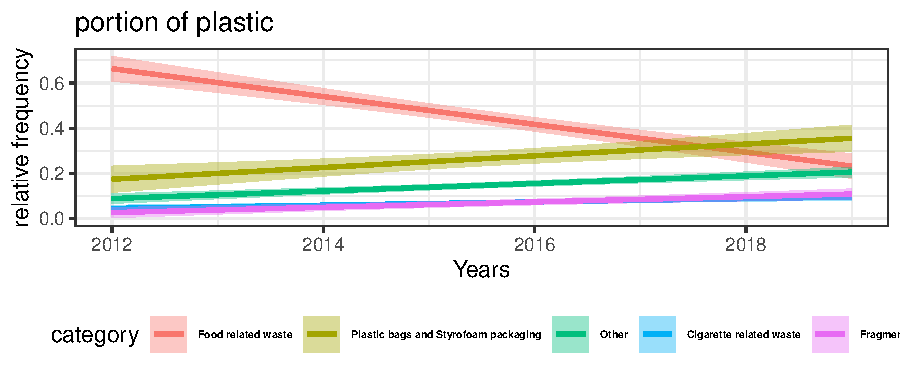
\includegraphics[width=1\linewidth]{figure/unnamed-chunk-25-1} 

\end{knitrout}
\caption {Some sort of caption here}
\label{figG1}
\end {center}
\end {figure}


We see here a graphical representation of the relative frequency of the 5 different categories of plastic debris over the years. The hint we are getting here is that "Cigarette realted waste, "Food related waste", "Fragments" seem to experiance some change, whereas "Other" and Plastic bags and styrofoam packaging" seem to remain steady. We go on and create a model and test it on untrained data to see if what is the actual case.


\begin{knitrout}\small
\definecolor{shadecolor}{rgb}{0.969, 0.969, 0.969}\color{fgcolor}\begin{kframe}
\begin{alltt}
\hlcom{#1/4/20}
\hlcom{### MODELING with new categorisation}


\hlcom{# create train and test set}
\hlstd{n} \hlkwb{<-} \hlkwd{nrow}\hlstd{(dfTotN)}  \hlcom{# Number of observations}
\hlstd{ntrain} \hlkwb{<-} \hlkwd{round}\hlstd{(n}\hlopt{*}\hlnum{0.75}\hlstd{)}  \hlcom{# 75% for training set}
\hlkwd{set.seed}\hlstd{(}\hlnum{314}\hlstd{)}    \hlcom{# Set seed for reproducible results}
\hlstd{tindex} \hlkwb{<-} \hlkwd{sample}\hlstd{(n, ntrain)}   \hlcom{# Create a random index}
\hlstd{train_dfTotN} \hlkwb{<-} \hlstd{dfTotN[tindex,]}   \hlcom{# Create training set}
\hlstd{test_dfTotN} \hlkwb{<-} \hlstd{dfTotN[}\hlopt{-}\hlstd{tindex,]}

\hlcom{# modelling for category "Cigarette related waste"}

\hlstd{train_Cigrel} \hlkwb{<-} \hlstd{train_dfTotN} \hlopt
  \hlkwd{filter}\hlstd{(category}\hlopt{==}\hlstr{"Cigarette related waste"}\hlstd{)} \hlopt
  \hlkwd{group_by}\hlstd{(year)}

\hlstd{test_Cigrel} \hlkwb{<-} \hlstd{test_dfTotN} \hlopt
  \hlkwd{filter}\hlstd{(category}\hlopt{==}\hlstr{"Cigarette related waste"}\hlstd{)} \hlopt
  \hlkwd{group_by}\hlstd{(year)}

\hlkwd{set.seed}\hlstd{(}\hlnum{1234}\hlstd{)}
\hlstd{train_Cigrel.modelN} \hlkwb{<-} \hlkwd{lm}\hlstd{(freq} \hlopt{~} \hlstd{year,} \hlkwc{data} \hlstd{= train_Cigrel)}
\hlkwd{summary}\hlstd{(train_Cigrel.modelN)}
\end{alltt}
\begin{verbatim}
## 
## Call:
## lm(formula = freq ~ year, data = train_Cigrel)
## 
## Residuals:
##      Min       1Q   Median       3Q      Max 
## -0.06059 -0.02546 -0.00721  0.01012  0.20490 
## 
## Coefficients:
##               Estimate Std. Error t value Pr(>|t|)   
## (Intercept) -15.866832   4.775446  -3.323  0.00146 **
## year          0.007910   0.002369   3.338  0.00139 **
## ---
## Signif. codes:  0 '***' 0.001 '**' 0.01 '*' 0.05 '.' 0.1 ' ' 1
## 
## Residual standard error: 0.04331 on 66 degrees of freedom
## Multiple R-squared:  0.1444,	Adjusted R-squared:  0.1315 
## F-statistic: 11.14 on 1 and 66 DF,  p-value: 0.00139
\end{verbatim}
\begin{alltt}
\hlkwd{print}\hlstd{(}\hlstr{"PREDICTION"}\hlstd{)}
\end{alltt}
\begin{verbatim}
## [1] "PREDICTION"
\end{verbatim}
\begin{alltt}
\hlstd{pred_Cigrel} \hlkwb{<-} \hlkwd{predict}\hlstd{(train_Cigrel.modelN, test_Cigrel)}
\hlkwd{summary}\hlstd{(pred_Cigrel)}
\end{alltt}
\begin{verbatim}
##    Min. 1st Qu.  Median    Mean 3rd Qu.    Max. 
## 0.04720 0.06301 0.07092 0.07714 0.09465 0.10256
\end{verbatim}
\begin{alltt}
\hlstd{actuals_predsCigrel} \hlkwb{<-} \hlkwd{data.frame}\hlstd{(}\hlkwd{cbind}\hlstd{(}\hlkwc{actuals}\hlstd{=test_Cigrel}\hlopt{$}\hlstd{freq,} \hlkwc{predicteds}\hlstd{=pred_Cigrel))}
\hlkwd{head}\hlstd{(actuals_predsCigrel)}
\end{alltt}
\begin{verbatim}
##      actuals predicteds
## 1 0.05109361 0.04719559
## 2 0.05814490 0.04719559
## 3 0.03971631 0.04719559
## 4 0.03750621 0.05510514
## 5 0.01202405 0.05510514
## 6 0.05699357 0.05510514
\end{verbatim}
\begin{alltt}
\hlstd{correlation_accuracy} \hlkwb{<-} \hlkwd{cor}\hlstd{(actuals_predsCigrel)}
\hlstd{min_max_accuracy} \hlkwb{<-} \hlkwd{mean}\hlstd{(}\hlkwd{apply}\hlstd{(actuals_predsCigrel,} \hlnum{1}\hlstd{, min)} \hlopt{/} \hlkwd{apply}\hlstd{(actuals_predsCigrel,} \hlnum{1}\hlstd{, max))}

\hlstd{mape} \hlkwb{<-} \hlkwd{mean}\hlstd{(}\hlkwd{abs}\hlstd{((actuals_predsCigrel}\hlopt{$}\hlstd{predicteds} \hlopt{-} \hlstd{actuals_predsCigrel}\hlopt{$}\hlstd{actuals))}\hlopt{/}\hlstd{actuals_predsCigrel}\hlopt{$}\hlstd{actuals)}

\hlstd{correlation_accuracy}
\end{alltt}
\begin{verbatim}
##              actuals predicteds
## actuals    1.0000000  0.5444291
## predicteds 0.5444291  1.0000000
\end{verbatim}
\begin{alltt}
\hlstd{min_max_accuracy}
\end{alltt}
\begin{verbatim}
## [1] 0.7259542
\end{verbatim}
\begin{alltt}
\hlstd{mape}
\end{alltt}
\begin{verbatim}
## [1] 0.7522119
\end{verbatim}
\end{kframe}
\end{knitrout}


\begin{knitrout}\small
\definecolor{shadecolor}{rgb}{0.969, 0.969, 0.969}\color{fgcolor}\begin{kframe}
\begin{alltt}
\hlcom{# modelling for category "Food related waste"}

\hlstd{train_Foodrel} \hlkwb{<-} \hlstd{train_dfTotN} \hlopt
  \hlkwd{filter}\hlstd{(category}\hlopt{==}\hlstr{"Food related waste"}\hlstd{)} \hlopt
  \hlkwd{group_by}\hlstd{(year)}

\hlstd{test_Foodrel} \hlkwb{<-} \hlstd{test_dfTotN} \hlopt
  \hlkwd{filter}\hlstd{(category}\hlopt{==}\hlstr{"Food related waste"}\hlstd{)} \hlopt
  \hlkwd{group_by}\hlstd{(year)}

\hlkwd{set.seed}\hlstd{(}\hlnum{1234}\hlstd{)}
\hlstd{train_Foodrel.modelN} \hlkwb{<-} \hlkwd{lm}\hlstd{(freq} \hlopt{~} \hlstd{year,} \hlkwc{data} \hlstd{= train_Foodrel)}
\hlkwd{summary}\hlstd{(train_Foodrel.modelN)}
\end{alltt}
\begin{verbatim}
## 
## Call:
## lm(formula = freq ~ year, data = train_Foodrel)
## 
## Residuals:
##      Min       1Q   Median       3Q      Max 
## -0.50287 -0.07168 -0.00561  0.10218  0.34829 
## 
## Coefficients:
##               Estimate Std. Error t value Pr(>|t|)    
## (Intercept) 118.166588  15.395217   7.676 5.31e-11 ***
## year         -0.058414   0.007638  -7.647 6.00e-11 ***
## ---
## Signif. codes:  0 '***' 0.001 '**' 0.01 '*' 0.05 '.' 0.1 ' ' 1
## 
## Residual standard error: 0.1541 on 74 degrees of freedom
## Multiple R-squared:  0.4414,	Adjusted R-squared:  0.4339 
## F-statistic: 58.48 on 1 and 74 DF,  p-value: 5.998e-11
\end{verbatim}
\begin{alltt}
\hlkwd{print}\hlstd{(}\hlstr{"PREDICTION"}\hlstd{)}
\end{alltt}
\begin{verbatim}
## [1] "PREDICTION"
\end{verbatim}
\begin{alltt}
\hlstd{pred_Foodrel} \hlkwb{<-} \hlkwd{predict}\hlstd{(train_Foodrel.modelN, test_Foodrel)}
\hlkwd{summary}\hlstd{(pred_Foodrel)}
\end{alltt}
\begin{verbatim}
##    Min. 1st Qu.  Median    Mean 3rd Qu.    Max. 
##  0.2292  0.3314  0.4921  0.4395  0.5213  0.6381
\end{verbatim}
\begin{alltt}
\hlstd{actuals_predsFoodrel} \hlkwb{<-} \hlkwd{data.frame}\hlstd{(}\hlkwd{cbind}\hlstd{(}\hlkwc{actuals}\hlstd{=test_Foodrel}\hlopt{$}\hlstd{freq,} \hlkwc{predicteds}\hlstd{=pred_Foodrel))}
\hlkwd{head}\hlstd{(actuals_predsFoodrel)}
\end{alltt}
\begin{verbatim}
##     actuals predicteds
## 1 0.9761681  0.6381043
## 2 0.6351528  0.5796905
## 3 0.5822665  0.5796905
## 4 0.7911040  0.5796905
## 5 0.4837153  0.5212767
## 6 0.5395366  0.5212767
\end{verbatim}
\begin{alltt}
\hlstd{correlation_accuracy} \hlkwb{<-} \hlkwd{cor}\hlstd{(actuals_predsFoodrel)}
\hlstd{min_max_accuracy} \hlkwb{<-} \hlkwd{mean}\hlstd{(}\hlkwd{apply}\hlstd{(actuals_predsFoodrel,} \hlnum{1}\hlstd{, min)} \hlopt{/} \hlkwd{apply}\hlstd{(actuals_predsFoodrel,} \hlnum{1}\hlstd{, max))}
\hlcom{# => 53.73%, min_max accuracy}
\hlstd{mape} \hlkwb{<-} \hlkwd{mean}\hlstd{(}\hlkwd{abs}\hlstd{((actuals_predsFoodrel}\hlopt{$}\hlstd{predicteds} \hlopt{-} \hlstd{actuals_predsFoodrel}\hlopt{$}\hlstd{actuals))}\hlopt{/}\hlstd{actuals_predsFoodrel}\hlopt{$}\hlstd{actuals)}

\hlstd{correlation_accuracy}
\end{alltt}
\begin{verbatim}
##              actuals predicteds
## actuals    1.0000000  0.8537377
## predicteds 0.8537377  1.0000000
\end{verbatim}
\begin{alltt}
\hlstd{min_max_accuracy}
\end{alltt}
\begin{verbatim}
## [1] 0.8523448
\end{verbatim}
\begin{alltt}
\hlstd{mape}
\end{alltt}
\begin{verbatim}
## [1] 0.1546258
\end{verbatim}
\begin{alltt}
\hlcom{# modelling for category "Other"}
\hlstd{train_Other} \hlkwb{<-} \hlstd{train_dfTotN} \hlopt
  \hlkwd{filter}\hlstd{(category}\hlopt{==}\hlstr{"Other"}\hlstd{)} \hlopt
  \hlkwd{group_by}\hlstd{(year)}

\hlstd{test_Other} \hlkwb{<-} \hlstd{test_dfTotN} \hlopt
  \hlkwd{filter}\hlstd{(category}\hlopt{==}\hlstr{"Other"}\hlstd{)} \hlopt
  \hlkwd{group_by}\hlstd{(year)}

\hlkwd{set.seed}\hlstd{(}\hlnum{1234}\hlstd{)}
\hlstd{train_Other.modelN} \hlkwb{<-} \hlkwd{lm}\hlstd{(freq} \hlopt{~} \hlstd{year,} \hlkwc{data} \hlstd{= train_Other)}
\hlkwd{summary}\hlstd{(train_Other.modelN)}
\end{alltt}
\begin{verbatim}
## 
## Call:
## lm(formula = freq ~ year, data = train_Other)
## 
## Residuals:
##       Min        1Q    Median        3Q       Max 
## -0.131735 -0.041328 -0.005655  0.035206  0.134108 
## 
## Coefficients:
##               Estimate Std. Error t value Pr(>|t|)    
## (Intercept) -33.991092   6.112772  -5.561 4.73e-07 ***
## year          0.016938   0.003033   5.585 4.30e-07 ***
## ---
## Signif. codes:  0 '***' 0.001 '**' 0.01 '*' 0.05 '.' 0.1 ' ' 1
## 
## Residual standard error: 0.06088 on 69 degrees of freedom
## Multiple R-squared:  0.3113,	Adjusted R-squared:  0.3013 
## F-statistic: 31.19 on 1 and 69 DF,  p-value: 4.296e-07
\end{verbatim}
\begin{alltt}
\hlkwd{print}\hlstd{(}\hlstr{"PREDICTION"}\hlstd{)}
\end{alltt}
\begin{verbatim}
## [1] "PREDICTION"
\end{verbatim}
\begin{alltt}
\hlstd{pred_Other} \hlkwb{<-} \hlkwd{predict}\hlstd{(train_Other.modelN, test_Other)}
\hlkwd{summary}\hlstd{(pred_Other)}
\end{alltt}
\begin{verbatim}
##    Min. 1st Qu.  Median    Mean 3rd Qu.    Max. 
## 0.08807 0.12195 0.13889 0.14228 0.17276 0.20664
\end{verbatim}
\begin{alltt}
\hlstd{actuals_predsOther} \hlkwb{<-} \hlkwd{data.frame}\hlstd{(}\hlkwd{cbind}\hlstd{(}\hlkwc{actuals}\hlstd{=test_Other}\hlopt{$}\hlstd{freq,} \hlkwc{predicteds}\hlstd{=pred_Other))}
\hlkwd{head}\hlstd{(actuals_predsOther)}
\end{alltt}
\begin{verbatim}
##      actuals predicteds
## 1 0.05367366 0.08807451
## 2 0.13682008 0.08807451
## 3 0.26636312 0.10501246
## 4 0.10336403 0.10501246
## 5 0.05515197 0.10501246
## 6 0.14156627 0.10501246
\end{verbatim}
\begin{alltt}
\hlstd{correlation_accuracy} \hlkwb{<-} \hlkwd{cor}\hlstd{(actuals_predsOther)}  \hlcom{# 5.31%}
\hlstd{min_max_accuracy} \hlkwb{<-} \hlkwd{mean}\hlstd{(}\hlkwd{apply}\hlstd{(actuals_predsOther,} \hlnum{1}\hlstd{, min)} \hlopt{/} \hlkwd{apply}\hlstd{(actuals_predsOther,} \hlnum{1}\hlstd{, max))}
\hlstd{mape} \hlkwb{<-} \hlkwd{mean}\hlstd{(}\hlkwd{abs}\hlstd{((actuals_predsOther}\hlopt{$}\hlstd{predicteds} \hlopt{-} \hlstd{actuals_predsOther}\hlopt{$}\hlstd{actuals))}\hlopt{/}\hlstd{actuals_predsOther}\hlopt{$}\hlstd{actuals)}

\hlstd{correlation_accuracy}
\end{alltt}
\begin{verbatim}
##              actuals predicteds
## actuals    1.0000000  0.4983376
## predicteds 0.4983376  1.0000000
\end{verbatim}
\begin{alltt}
\hlstd{min_max_accuracy}
\end{alltt}
\begin{verbatim}
## [1] 0.7441029
\end{verbatim}
\begin{alltt}
\hlstd{mape}
\end{alltt}
\begin{verbatim}
## [1] 0.354683
\end{verbatim}
\begin{alltt}
\hlcom{# modelling for category "Plastic bags and Styrofoam packaging"}
\hlstd{train_Plbag} \hlkwb{<-} \hlstd{train_dfTotN} \hlopt
  \hlkwd{filter}\hlstd{(category}\hlopt{==}\hlstr{"Plastic bags and Styrofoam packaging"}\hlstd{)} \hlopt
  \hlkwd{group_by}\hlstd{(year)}

\hlstd{test_Plbag} \hlkwb{<-} \hlstd{test_dfTotN} \hlopt
  \hlkwd{filter}\hlstd{(category}\hlopt{==}\hlstr{"Plastic bags and Styrofoam packaging"}\hlstd{)} \hlopt
  \hlkwd{group_by}\hlstd{(year)}

\hlkwd{set.seed}\hlstd{(}\hlnum{1234}\hlstd{)}
\hlstd{train_Plbag.modelN} \hlkwb{<-} \hlkwd{lm}\hlstd{(freq} \hlopt{~} \hlstd{year,} \hlkwc{data} \hlstd{= train_Plbag)}
\hlkwd{summary}\hlstd{(train_Plbag.modelN)}
\end{alltt}
\begin{verbatim}
## 
## Call:
## lm(formula = freq ~ year, data = train_Plbag)
## 
## Residuals:
##      Min       1Q   Median       3Q      Max 
## -0.31838 -0.09726 -0.02112  0.05326  0.66454 
## 
## Coefficients:
##               Estimate Std. Error t value Pr(>|t|)   
## (Intercept) -53.792345  16.802490  -3.201  0.00204 **
## year          0.026822   0.008336   3.217  0.00194 **
## ---
## Signif. codes:  0 '***' 0.001 '**' 0.01 '*' 0.05 '.' 0.1 ' ' 1
## 
## Residual standard error: 0.1608 on 72 degrees of freedom
## Multiple R-squared:  0.1257,	Adjusted R-squared:  0.1136 
## F-statistic: 10.35 on 1 and 72 DF,  p-value: 0.001939
\end{verbatim}
\begin{alltt}
\hlkwd{print}\hlstd{(}\hlstr{"PREDICTION"}\hlstd{)}
\end{alltt}
\begin{verbatim}
## [1] "PREDICTION"
\end{verbatim}
\begin{alltt}
\hlstd{pred_Plbag} \hlkwb{<-} \hlkwd{predict}\hlstd{(train_Plbag.modelN, test_Plbag)}
\hlkwd{summary}\hlstd{(pred_Plbag)}
\end{alltt}
\begin{verbatim}
##    Min. 1st Qu.  Median    Mean 3rd Qu.    Max. 
##  0.1732  0.2000  0.2536  0.2609  0.3341  0.3609
\end{verbatim}
\begin{alltt}
\hlstd{actuals_predsPlbag} \hlkwb{<-} \hlkwd{data.frame}\hlstd{(}\hlkwd{cbind}\hlstd{(}\hlkwc{actuals}\hlstd{=test_Plbag}\hlopt{$}\hlstd{freq,} \hlkwc{predicteds}\hlstd{=pred_Plbag))}
\hlkwd{head}\hlstd{(actuals_predsPlbag)}
\end{alltt}
\begin{verbatim}
##      actuals predicteds
## 1 0.12998318  0.1731621
## 2 0.14728033  0.1731621
## 3 0.08181818  0.1731621
## 4 0.13607595  0.1731621
## 5 0.28635887  0.1999839
## 6 0.06939979  0.1999839
\end{verbatim}
\begin{alltt}
\hlstd{correlation_accuracy} \hlkwb{<-} \hlkwd{cor}\hlstd{(actuals_predsPlbag)}  \hlcom{# 5.31%}
\hlstd{min_max_accuracy} \hlkwb{<-} \hlkwd{mean}\hlstd{(}\hlkwd{apply}\hlstd{(actuals_predsPlbag,} \hlnum{1}\hlstd{, min)} \hlopt{/} \hlkwd{apply}\hlstd{(actuals_predsPlbag,} \hlnum{1}\hlstd{, max))}
\hlstd{mape} \hlkwb{<-} \hlkwd{mean}\hlstd{(}\hlkwd{abs}\hlstd{((actuals_predsPlbag}\hlopt{$}\hlstd{predicteds} \hlopt{-} \hlstd{actuals_predsPlbag}\hlopt{$}\hlstd{actuals))}\hlopt{/}\hlstd{actuals_predsPlbag}\hlopt{$}\hlstd{actuals)}

\hlstd{correlation_accuracy}
\end{alltt}
\begin{verbatim}
##              actuals predicteds
## actuals    1.0000000  0.3534861
## predicteds 0.3534861  1.0000000
\end{verbatim}
\begin{alltt}
\hlstd{min_max_accuracy}
\end{alltt}
\begin{verbatim}
## [1] 0.6623657
\end{verbatim}
\begin{alltt}
\hlstd{mape}
\end{alltt}
\begin{verbatim}
## [1] 2.273597
\end{verbatim}
\begin{alltt}
\hlcom{# modelling for category "Fragments"}
\hlstd{train_Frag} \hlkwb{<-} \hlstd{train_dfTotN} \hlopt
  \hlkwd{filter}\hlstd{(category}\hlopt{==}\hlstr{"Fragments"}\hlstd{)} \hlopt
  \hlkwd{group_by}\hlstd{(year)}

\hlstd{test_Frag} \hlkwb{<-} \hlstd{test_dfTotN} \hlopt
  \hlkwd{filter}\hlstd{(category}\hlopt{==}\hlstr{"Fragments"}\hlstd{)} \hlopt
  \hlkwd{group_by}\hlstd{(year)}

\hlkwd{set.seed}\hlstd{(}\hlnum{1234}\hlstd{)}
\hlstd{train_Frag.modelN} \hlkwb{<-} \hlkwd{lm}\hlstd{(freq} \hlopt{~} \hlstd{year,} \hlkwc{data} \hlstd{= train_Frag)}
\hlkwd{summary}\hlstd{(train_Frag.modelN)}
\end{alltt}
\begin{verbatim}
## 
## Call:
## lm(formula = freq ~ year, data = train_Frag)
## 
## Residuals:
##      Min       1Q   Median       3Q      Max 
## -0.07328 -0.03075 -0.01469  0.01405  0.36377 
## 
## Coefficients:
##               Estimate Std. Error t value Pr(>|t|)   
## (Intercept) -21.074627   6.678746  -3.155  0.00237 **
## year          0.010490   0.003314   3.165  0.00230 **
## ---
## Signif. codes:  0 '***' 0.001 '**' 0.01 '*' 0.05 '.' 0.1 ' ' 1
## 
## Residual standard error: 0.06143 on 69 degrees of freedom
## Multiple R-squared:  0.1268,	Adjusted R-squared:  0.1142 
## F-statistic: 10.02 on 1 and 69 DF,  p-value: 0.002305
\end{verbatim}
\begin{alltt}
\hlkwd{print}\hlstd{(}\hlstr{"PREDICTION"}\hlstd{)}
\end{alltt}
\begin{verbatim}
## [1] "PREDICTION"
\end{verbatim}
\begin{alltt}
\hlstd{pred_Frag} \hlkwb{<-} \hlkwd{predict}\hlstd{(train_Frag.modelN, test_Frag)}
\hlkwd{summary}\hlstd{(pred_Frag)}
\end{alltt}
\begin{verbatim}
##    Min. 1st Qu.  Median    Mean 3rd Qu.    Max. 
## 0.03035 0.05133 0.07231 0.06812 0.09329 0.10378
\end{verbatim}
\begin{alltt}
\hlstd{actuals_predsFrag} \hlkwb{<-} \hlkwd{data.frame}\hlstd{(}\hlkwd{cbind}\hlstd{(}\hlkwc{actuals}\hlstd{=test_Frag}\hlopt{$}\hlstd{freq,} \hlkwc{predicteds}\hlstd{=pred_Frag))}
\hlkwd{head}\hlstd{(actuals_predsFrag)}
\end{alltt}
\begin{verbatim}
##        actuals predicteds
## 1 0.0006645432 0.03035393
## 2 0.0365704287 0.03035393
## 3 0.0420180954 0.03035393
## 4 0.0553760960 0.03035393
## 5 0.0240641711 0.03035393
## 6 0.0239271782 0.04084348
\end{verbatim}
\begin{alltt}
\hlstd{correlation_accuracy} \hlkwb{<-} \hlkwd{cor}\hlstd{(actuals_predsFrag)}  \hlcom{# 5.31%}
\hlstd{min_max_accuracy} \hlkwb{<-} \hlkwd{mean}\hlstd{(}\hlkwd{apply}\hlstd{(actuals_predsFrag,} \hlnum{1}\hlstd{, min)} \hlopt{/} \hlkwd{apply}\hlstd{(actuals_predsFrag,} \hlnum{1}\hlstd{, max))}
\hlstd{mape} \hlkwb{<-} \hlkwd{mean}\hlstd{(}\hlkwd{abs}\hlstd{((actuals_predsFrag}\hlopt{$}\hlstd{predicteds} \hlopt{-} \hlstd{actuals_predsFrag}\hlopt{$}\hlstd{actuals))}\hlopt{/}\hlstd{actuals_predsFrag}\hlopt{$}\hlstd{actuals)}

\hlstd{correlation_accuracy}
\end{alltt}
\begin{verbatim}
##              actuals predicteds
## actuals    1.0000000  0.4961031
## predicteds 0.4961031  1.0000000
\end{verbatim}
\begin{alltt}
\hlstd{min_max_accuracy}
\end{alltt}
\begin{verbatim}
## [1] 0.5303913
\end{verbatim}
\begin{alltt}
\hlstd{mape}
\end{alltt}
\begin{verbatim}
## [1] 2.69393
\end{verbatim}
\end{kframe}
\end{knitrout}

In total we see that time is statistically significant in the change of proportions of certain categories
of plastic waste: "cigarette related waste", "food related waste", "fragments". This is not the case for the "Other" and "Plastic bags and Styrofoam packaging" .
Some plastic waste categories are time variant while others aren't and this has to do a  lot with sampling techniques and one-sidedness of datasets. It does not mean that the datasets are wrong it just shows even more that what we have talked about over many group meetings regarding the dataset being biased one way or the other is clearly backed by statistical evidence within this dataset and by referencial evidence too."

"Paper: Spatial and Temporal Patterns of Stranded Intertidal Marine Debris:
Is There a Picture of Global Change?"


\begin{knitrout}\small
\definecolor{shadecolor}{rgb}{0.969, 0.969, 0.969}\color{fgcolor}\begin{kframe}
\begin{alltt}
\hlstd{plastic_category} \hlkwb{<-}\hlstd{(}\hlkwd{c}\hlstd{(}\hlstr{"cigarette related waste"}\hlstd{,} \hlstr{"food related waste"}\hlstd{,}\hlstr{"Fragments"}\hlstd{,} \hlstr{"Other"}\hlstd{,}\hlstr{"Plastic bags and Styrofoam packaging"} \hlstd{))}
\hlstd{slope_scores} \hlkwb{<-} \hlkwd{c}\hlstd{(}\hlopt{-}\hlnum{0.05512}\hlstd{,}\hlnum{0.030425}\hlstd{,} \hlnum{0.030950}\hlstd{,}\hlopt{-}\hlnum{0.002428}\hlstd{,}\hlopt{-}\hlnum{0.001151}\hlstd{)}
\hlstd{slope_interpretation} \hlkwb{<-}\hlkwd{c}\hlstd{(}\hlstr{"downward"}\hlstd{,} \hlstr{"upward"}\hlstd{,} \hlstr{"upward"}\hlstd{,} \hlstr{"relatively steady"}\hlstd{,} \hlstr{"relatively steady"}\hlstd{)}
\hlstd{p_value}\hlkwb{<-}\hlkwd{c}\hlstd{(}\hlstr{"<0.05"}\hlstd{,}\hlstr{"<0.05"}\hlstd{,}\hlstr{"<0.05"}\hlstd{,} \hlstr{">0.05"}\hlstd{,}\hlstr{">0.05"}\hlstd{)}
\hlstd{corr_accuracy}\hlkwb{<-}\hlkwd{c}\hlstd{(}\hlnum{0.62}\hlstd{,} \hlnum{0.35}\hlstd{,}\hlnum{0.48}\hlstd{,} \hlnum{0.27}\hlstd{,}\hlnum{0.38}\hlstd{)}
\hlstd{min_max_Acc}\hlkwb{<-}\hlkwd{c}\hlstd{(}\hlnum{0.67}\hlstd{,}\hlnum{0.72}\hlstd{,}\hlnum{0.67}\hlstd{,} \hlnum{0.65} \hlstd{,}\hlnum{0.67}\hlstd{)}
\hlstd{MAPE_scores}\hlkwb{<-}\hlkwd{c}\hlstd{(}\hlnum{0.99}\hlstd{,}\hlnum{0.91}\hlstd{,}\hlnum{0.54}\hlstd{,} \hlnum{0.89}\hlstd{,} \hlnum{0.43}\hlstd{)}
\hlstd{score_table} \hlkwb{<-} \hlkwd{data.frame}\hlstd{(plastic_category, p_value,slope_scores, slope_interpretation, corr_accuracy,min_max_Acc, MAPE_scores)}
\hlstd{score_table}
\end{alltt}
\begin{verbatim}
##                       plastic_category p_value slope_scores
## 1              cigarette related waste   <0.05    -0.055120
## 2                   food related waste   <0.05     0.030425
## 3                            Fragments   <0.05     0.030950
## 4                                Other   >0.05    -0.002428
## 5 Plastic bags and Styrofoam packaging   >0.05    -0.001151
##   slope_interpretation corr_accuracy min_max_Acc MAPE_scores
## 1             downward          0.62        0.67        0.99
## 2               upward          0.35        0.72        0.91
## 3               upward          0.48        0.67        0.54
## 4    relatively steady          0.27        0.65        0.89
## 5    relatively steady          0.38        0.67        0.43
\end{verbatim}
\end{kframe}
\end{knitrout}

On metrics used:
$Pr(>|t|)$ is the p-value, defined as the probability of observing any value equal or larger than t if H0 is true. The larger the t statistic, the smaller the p-value. Generally, we use 0.05 as the cutoff for significance. When p-values are smaller than 0.05, we reject H0 that there's no difference between the means and conclude that a significant difference does exist. If the p-value is larger than 0.05, we cannot conclude that a significant difference exists. P-value<0.05 means that there is statistical significance in the results presented. If p-value>0.05 we can not conclude on the statistical significance. 

Correlation accuracy:
A simple correlation between the actuals and predicted values can be used as a form of accuracy measure.
A higher correlation accuracy implies that the actuals and predicted values have similar directional movement, i.e. when the actuals values increase the predicted values also increase and vice-versa.

MinMax Accuracy:
MinMax tells you how far the model's prediction is off. For a perfect model, this measure is 1.0. The lower the measure, the worse the model, based on out-of-sample performance.
min\_max\_accuracy

MAPE:
The mean absolute percentage error (MAPE) is a statistical measure of how accurate a forecast system is. It measures this accuracy as a percentage, and can be calculated as the average absolute percent error for each time period minus actual values divided by actual values. 
eg a MAPE value of 0.99 states that our model's predictions are, on average, 0.99\% off from actual value.

On values of metrics used:
MinMax Accuracy is generally above 65\% but never exceeds 72\% for all cases, which means that the model does a moderate job in predicting accurately the relative frequency of each category over time.
The correlation accuracy is not that good which implies that the predicted values do not always follow the true values observed. The best value is for the model predicting on "cigarette related waste".
MAPE scores are pretty good for all models showing that no model's predictions are on average more than 1\% off from actual value. 




\subsection{Model Evaluation}


\subsection{Model Discussion}

As seen in the study of debris in a Eastern Mediterranean coastal town \cite{PORTMAN2017} the variability of non-plastic litter composition should make us aware that the local context must be taken into account. Perhaps, given that non-plastic litter is a hugely varying category, this way of thinking could be expanded into the plastic debris category of "Other", given that it is inherently varied let alone in a dataset that gathers information over the entire world. In fact, this could in reverse explain the higher p-value, since high variation within the category studied would yield results of insufficient trustworthiness. 

As mentioned in \cite{BROWNE2015} many intertidal sites seem to be transit areas for debris, with exports matching imports over time. This could hugely impact a created model especially given that in the dataset we used we didn't have such information available. It is also important to acknowledge that our dataset is Northamerican centred which and given that it has information gathered over a period of 10 years we cannot be sure of categorization biase in the data, since there is no proof of a single sampling protocol followed. We have already spotted one such occasion, rubber gloves, and taken care of it, but further study on it is needed. 


\pagebreak
\section{Discussion}

It was noted that the main system for reporting debris was used by large scale clobes. This means that data is not a continuous and even flow so during events such as international beach cleanup day there may be more data in the respective month. Since these events aim mostly to cleanup after big social events extra effort might have been made to retrive entertainment based debris such as fireworks, food packaging and six pack rings.The decrease in cigarette waste was theorised to be in corelation with a decreasing smoking rate however the cigarette waste was not the direct focus of this paper so that avenue of inquiry was not followed.






\section{Conclusion and Future Work}\label{cdsmote1}

The hypothesis H1 stands. This is no evidence as to a change in the percentage of marine debris being plastic in origin that can be observed in results such as in figure 4 which shows how the change in plastic quantity mirrors the change in overall debris quantity. \\

Future work might involve continuing to study corelations similar to the fireworks/july corelation that was discussed in section 4.3. Another line of study might be for example to compare the decreasing rate of cigarette use with the decreasing observtion of cigarette debris which had been observed over the years to see if there is a corollation there which was hypothosised but never investigated due to not being the direct inquiry of the report.     

Roshi's text below\\
4. Conclusion and Future WorkFrom our results and previous literature, it can clearly be seen that plastic is the mostabundant litter in the marine environment globally. Plastic was included in the 68\% of theobservations recorded and it made up of over 70\% of the quantity of debris that was recorded.Our results also indicate the successful use of citizen science projects to monitor marinepollution. There are various ways citizen science projects have been used for and here wefocused on distribution and composition of marine litter on a global scale. Identifying theamount and type of debris can help in identifying the sources of pollution. This can then helpeveryone to find out ways to reduce the source in the first place. We confirm the findings thatplastic is the main polluter in the marine environment and more needs to be done to reducethe plastic waste. Event driven pollution such as fireworks also plays a role in marinepollution and this can be reduced by raising awareness amongst the public and trying to findmore sustainable ways of celebrating events. The fact that plastic composition does notchange over time is also quite alarming. Although there have been a lot of awarenessprogrammes in the last decades, more needs to be done to see these changes that can reducethe damage done by plastic pollution.  \\

Future work can include looking at the marine pollution debris in smaller scale by regions.Each region is different and there are various factors that can affect the data observationssuch as the frequency of data submissions are not at the same time everywhere.  Since MDTis more focused on North America, this opportunity might be used to educate about it in otherregions of the world. Although we will never be able to identify the real sources of pollution,it can help in raising awareness of the damage done by plastic pollution in the marineenvironment and make the public more environmentally conscious. Regulations to discouragesingle used plastic items and smoking in public places have been enforced in many countries.It would be interesting to look at the effect these are having on the marine debris pollutionworldwide. However, more time and data will be required to see the change at a global scale. \\

Lots of beach clean ups and litter collections are done in the beaches worldwide to estimatethe marine pollution. However, the majority (70\%) of the marine debris are not on the surfacebut on the seafloor  (UNEP, 2005).  More research and studies are needed to accuratelyestimate the pollution in our oceans. Although marine pollution is a global issue, more needto be done locally to reduce the sources of the pollution. In addition, standardised monitoring protocol and global partnerships are   essential for efficient management of marine plasticpollution. \\

\hl{reference: United Nations Environment Programme (2005). Annual Evaluation Report.}



\pagebreak
\section{Project Management}\label{mgt}
\subsection{Facilities}
Group 2 communicated using a dedicated Slack Channel, Github repository and weekly 1 hour meetings before the wednesday lab.
All project documents used and the final report can be accessed from the \textit{\href{https://github.com/KarenJewell/CMM507Group2}{Public Github Repository}}
\hl{obviously we need to mention the whole covid-19 thing and how we worked around it.}

\subsection{Project Progress}

% Pay attention to the code below including the chunk options 
\begin{kframe}
\begin{alltt}
\hlkwd{require}\hlstd{(openxlsx);}
\hlkwd{require}\hlstd{(readxl)}
\hlkwd{library}\hlstd{(stringr);}\hlkwd{library}\hlstd{(data.table)}
\hlkwd{library}\hlstd{(XLConnect)}
\hlkwd{library}\hlstd{(xtable)}

\hlcom{# Sheets names }
\hlstd{fileName} \hlkwb{<-} \hlstr{'data/meetings.xlsx'}
\hlstd{sheets} \hlkwb{<-} \hlstd{readxl}\hlopt{::}\hlkwd{excel_sheets}\hlstd{(fileName)}
\hlcom{#length(sheets)}
\hlcom{# Read 1st sheet (you shouldn't have more than one sheet for this task)}
\hlcom{# read sheet into dataframe, and rbind}
\hlstd{dfs} \hlkwb{<-} \hlkwd{readWorksheet}\hlstd{(}\hlkwd{loadWorkbook}\hlstd{(}\hlstr{"data/meetings.xlsx"}\hlstd{),}\hlkwc{sheet}\hlstd{=}\hlnum{1}\hlstd{)}
\hlstd{dfs}\hlopt{$}\hlstd{Date} \hlkwb{<-}\hlkwd{as.character}\hlstd{(dfs}\hlopt{$}\hlstd{Date)}
\hlkwd{print}\hlstd{(}\hlkwd{xtable}\hlstd{(dfs,}
                    \hlkwc{caption} \hlstd{=} \hlstr{"Record of Team Meetings"}\hlstd{,}
                    \hlkwc{label} \hlstd{=} \hlstr{"tab:one"}\hlstd{,}
                    \hlkwc{table.placement} \hlstd{=} \hlstr{""}\hlstd{,}
                    \hlcom{# align changes subject to number of columns }
                    \hlkwc{align} \hlstd{=} \hlstr{"lllp\{8cm\}lllll"}\hlstd{),}\hlkwc{include.rownames}\hlstd{=}\hlnum{FALSE}\hlstd{,}
                    \hlkwc{caption.placement} \hlstd{=} \hlstr{"top"}\hlstd{)}
\end{alltt}
\end{kframe}% latex table generated in R 3.6.1 by xtable 1.8-4 package
% Sun May 10 16:41:45 2020
\begin{table}[ht]
\centering
\caption{Record of Team Meetings} 
\label{tab:one}
\begin{tabular}{llp{8cm}lllll}
  \hline
No & Date & Topic & Alex & Georgios & Karen & Roshi & Stuart \\ 
  \hline
1.00 & 2020-02-05 & Group Formation: set up communication channel in Slack and GitHub repository & yes & yes & yes & yes & yes \\ 
  2.00 & 2020-02-11 & Agreed topic of "Plastic Pollution", distributed research activity for week & yes & yes & yes & yes & yes \\ 
  3.00 & 2020-02-18 & Presented inividuals' research findings and discussed hypothesis & yes & yes & yes & yes & yes \\ 
  4.00 & 2020-02-25 & Decided on final dataset to use and hypothesis of "proportion of marine plastics pollution does not change over time" & yes & yes & yes & yes & yes \\ 
  5.00 & 2020-03-04 & Presentation draft agreed & yes & yes & yes & yes & yes \\ 
  6.00 & 2020-03-10 & Distributed section writing activity for week & yes & yes & yes & yes & yes \\ 
  7.00 & 2020-03-17 &  &  &  &  &  &  \\ 
  8.00 & 2020-03-24 &  &  &  &  &  &  \\ 
  9.00 & 2020-03-31 &  &  &  &  &  &  \\ 
  10.00 & 2020-04-07 &  &  &  &  &  &  \\ 
  11.00 & 2020-04-14 &  &  &  &  &  &  \\ 
  12.00 & 2020-04-21 &  &  &  &  &  &  \\ 
   \hline
\end{tabular}
\end{table}





\subsection{Peer-assessment}

\begin{kframe}
\begin{alltt}
\hlkwd{require}\hlstd{(openxlsx);}
\hlkwd{require}\hlstd{(readxl)}
\hlkwd{library}\hlstd{(stringr);}\hlkwd{library}\hlstd{(data.table)}
\hlkwd{library}\hlstd{(XLConnect)}
\hlkwd{library}\hlstd{(xtable)}

\hlcom{# Sheets names }
\hlstd{fileName} \hlkwb{<-} \hlstr{'data/peers.xlsx'}
\hlstd{sheets} \hlkwb{<-} \hlstd{readxl}\hlopt{::}\hlkwd{excel_sheets}\hlstd{(fileName)}
\hlcom{#length(sheets)}
\hlcom{# Read 1st sheet (you shouldn't have more than one sheet for this task)}
\hlcom{# read sheet into dataframe, and rbind}
\hlstd{dfs} \hlkwb{<-} \hlkwd{readWorksheet}\hlstd{(}\hlkwd{loadWorkbook}\hlstd{(}\hlstr{"data/peers.xlsx"}\hlstd{),}\hlkwc{sheet}\hlstd{=}\hlnum{1}\hlstd{)}

\hlcom{# convert fields into chars}
\hlstd{dfs[, ]} \hlkwb{<-} \hlkwd{lapply}\hlstd{(dfs[, ], as.character)}

\hlkwd{print}\hlstd{(}\hlkwd{xtable}\hlstd{(dfs,}
                    \hlkwc{caption} \hlstd{=} \hlstr{"Peer Assessment out of 100"}\hlstd{,}
                    \hlkwc{label} \hlstd{=} \hlstr{"tab:two"}\hlstd{,}
                    \hlkwc{table.placement} \hlstd{=} \hlstr{""}\hlstd{,}
                    \hlcom{# align changes subject to number of columns }
                    \hlkwc{align} \hlstd{=} \hlstr{"lllllll"}\hlstd{),}\hlkwc{include.rownames}\hlstd{=}\hlnum{FALSE}\hlstd{,}
                    \hlkwc{caption.placement} \hlstd{=} \hlstr{"top"}\hlstd{)}
\end{alltt}
\end{kframe}% latex table generated in R 3.6.1 by xtable 1.8-4 package
% Sun May 10 16:41:46 2020
\begin{table}[ht]
\centering
\caption{Peer Assessment out of 100} 
\label{tab:two}
\begin{tabular}{llllll}
  \hline
Peer.Review & Alex & Georgios & Karen & Roshi & Stuart \\ 
  \hline
Alex & 100 & 100 & 100 & 100 & 100 \\ 
  Georgios & 100 & 100 & 100 & 100 & 100 \\ 
  Karen & 100 & 100 & 100 & 100 & 100 \\ 
  Roshi & 100 & 100 & 100 & 100 & 100 \\ 
  Stuart & 100 & 100 & 100 & 100 & 100 \\ 
   \hline
\end{tabular}
\end{table}



\pagebreak
\section*{References}\label{pubs}
\printbibliography[heading=none]

\end{document}
